\documentclass[a4paper,11pt]{report}

\usepackage{parskip}
\usepackage[margin=2.54cm]{geometry}
\usepackage[utf8]{inputenc}
\usepackage{graphicx}
\usepackage[table,xcdraw]{xcolor} 
\usepackage{pdfpages}  %to insert pdf documents
\usepackage[draft]{todonotes}
\usepackage{pdflscape}
\usepackage{teresa}  % this is the project-layout style

%Joao Imports
\usepackage{framed,color}
\definecolor{shadecolor}{rgb}{0.9,0.9,0.9}
\usepackage[hidelinks]{hyperref}
\usepackage[hyphenbreaks]{breakurl}
\usepackage{multirow}
\usepackage{subcaption}
\usepackage{amsfonts}
\usepackage{amsmath}
\usepackage{amsthm}
\usepackage{amssymb}

\DeclareMathOperator*{\argmin}{\arg\!\min} 
\DeclareMathOperator*{\argmax}{\arg\!\max}
\usepackage{mathtools}
\usepackage{algorithm}
\usepackage{algorithmic}
\renewcommand{\rmdefault}{phv} % Arial
\renewcommand{\sfdefault}{phv} % Arial
 \usepackage[T1]{fontenc}

\graphicspath{{./}{figures/}}
%\theoremstyle{remark}
\newtheorem{req}{Requirement}
%\newcommand{\citn}{\begin{footnotesize}[cit. needed]\end{footnotesize}}
%\newcommand{\sw}[1]{\textcolor{red}{SW: #1}}
%\newcommand{\jtodo}[1]{\todo[inline]{TODO (Joao): #1}}
\newcommand{\halfrule}{\begin{center}{\rule{0.5\textwidth}{.4pt}}\end{center}}
\newenvironment{draftpts}
{\noindent\ignorespaces\begin{shaded}\begin{center}\footnotesize{DRAFT | Topics to include:}\end{center}\begin{small}}
{\end{small}\end{shaded}\par\noindent\ignorespacesafterend}

\setcounter{secnumdepth}{5}
\setcounter{tocdepth}{5}

%% Adapt the version and code to your deliverable.
%% Those values will appear in the header
\delivcode{D5.3}
\title{Feedback Part 2\\ Integrated Feedback System}
%% Running title
\titlefoot{Feedback Part 2 -- Integrated Feedback System}

\duedate{M30 -  May  31, 2016}
\wpleader{UvA}
\security{Public} %Public or private
\status{Submitted} %Submitted
\delivversion{1.0}



\begin{document}

\maketitle
\makeheader


%%Add a new row with the current version info. 
\begin{documentinfo}

\begin{tabular}{|p{5cm}|p{4cm}|p{5cm}|}
        \hline
        \rowcolor{gray!50}
        Date and Version Number & Author & Comments\\ \hline
        31.05.2016 v1.0 & Jo\~ao Messias \&\hfill Kyriacos Shiarlis & Initial Verson.\\ \hline
\end{tabular}

\end{documentinfo}


\pagebreak
\pagebreak

\tableofcontents

\pagebreak

\listoffigures

\pagebreak

\listoftables

\pagebreak

%\begin{abstract}

%\end{abstract}


\section{Executive Summary}\label{sec:sum}

The TERESA project aims to develop methods that allow a robot to interact effectively with a dynamic social environment. Specifically, we aim to place a semi-autonomous telepresence robot in a day-care center, to allow accessible and seamless communication between its members and remote visitors such as friends and family.\\

 A significant aspect of the project is that cost functions directly related to the movement and behaviour of the robot such as navigation and body pose are partly learned from data instead of being hard-coded. To make this possible, a variety of resources is required such as perception modules, learning algorithms, and of course the data themselves. \\

This deliverable describes the latest advancements 
elements for the TERESA robot through human feedback, in compliance with the 
Description of Work. It discusses:

\begin{itemize}
  \item Learning Algorithms. These are the methods that allow us to associate data from different sensors with feedback from the experiment subjects, into a cost function. We describe the algorithms used and methods for choosing between different design decisions within each algorithm.
  \item Experimentation. We perform experiments with manually 
controlled robots in which the involved subject thinks are autonomous. We describe 
specific instances of such a method, both for social navigation and social conversation scenario, where a 
  large amount of data and human feedback is collected and processed.
  \item Implementation. Using our methods, the collected data and existing algorithms we perform learning in real and simulated robot settings.
\end{itemize}

We present results and progress for all the above topics and explain in what 
ways their respective performance can be improved in the future.

\section{Contributors}\label{sec:cont}

The main contributors to this document are Kyriacos Shiarlis (UvA), Richard Pronk (UvA), Jo\~{a}o Messias (UvA) and Shimon Whiteson (UOXF). The document was reviewed by Luis Merino and Jes\'{u}s Capit\'{a}n (UPO).

\newpage

\section{Introduction}\label{sec:intro}

The technical goal of TERESA is to develop technology that enables a semi-autonomous robot to behave in an acceptable way in social situations. However, it is very hard to determine explicitly what constitutes an “acceptable way” for a robot to behave. This statement acts as motivation in this project, which aims to overcome this difficulty through learning. Work Package 5, and hence this deliverable, is mainly concerned with this idea of learning the correct behaviour from various feedback signals. Specifically, the robot should be able to learn from examples of human controller and from implicit or explicit feedback from people controlling or interacting with the robot.

An important method for teaching a robot a desired behaviour is Inverse Reinforcement Learning (IRL) \cite{abbeel2004apprenticeship}, which was further described in detail in \cite{d5.1} . IRL uses data from succesful demonstrations of a task to learn an expert's underlying \emph{cost function}. This cost function is then used to determine the robots behaviour in new situations. This deliverable offers two contributions to IRL, with social robotics being a strong application focus.

The first contribution is an algorithm we call inverse reinforcement learning from failure (IRLF) and is described in Section \ref{sec:irlf}. The method extends IRL, allowing it to learn from data of both succesful and \emph{failed} demonstrations of a task. Experiments on both simulated and real robot data demonstrate that IRLF converges faster and generalises better than methods that do not use this extra source of data, especially when few successful demonstrations are available. 

Our second contribution to IRL is described in Section \ref{sec:rrt-iros} and focuses on the task of social navigation. Social navigation is typically a very hard problem to model using standard IRL methods. However the key characteristic of IRL, i.e., learning cost functions from demonstration, is extremely appealing. Using the strengths and shortcomings of IRL as motivation, we develop Rapidly Exploring Learning Trees (RLT$^*$). The algorithm allows us to learn cost functions for conventional and widely used robotic path planners called Rapidly Exploring Random Trees (RRT$^*$). We describe our algorithm in detail and perform experimental comparisons with other learning algorithms, showing clear improvement in terms of both speed and learning capability.

A social telepresence robot, must not only be capable of navigating to a target location in a socially normative manner, but also interact with people in an equally appropriate fashion. For example when interacting with a person the robot must keep an appropriate distance and when interacting with a group, it must make sure that it is orientated in a way, such that no person within the group feels excluded. In Section \ref{sec:cost_functions} we show how these cost functions for these behaviours are learned using supervised learning. We describe how appropriate data of interaction and feedback was collected and how this was used to improve upon the social capabilities of the TERESA robot.

\section{Inverse Reinforcement Learning from Failure}
\label{sec:irlf}

In IRL \cite{ng2000algorithms}, an \emph{apprentice} aims to learn a policy for acting in an environment, typically modelled as a \emph{Markov decision process} (MDP), for which the reward function is not available, but successful demonstrations provided by an \emph{expert} performing the task are given instead. An IRL algorithm tries to find a reward function that leads the apprentice to behave  similarly to the expert while generalising well to situations for which expert data are not available. Social robotic behaviour is an excellent example of an application where a behaviour can be easily demonstrated, but not easily coded. Therefore, any progress in IRL is bound to greatly benefit the applications which we are considering in the TERESA project.

%Numerous IRL methods have been developed, using structured prediction \cite{klein2012inverse,ratliff2006maximum}, Bayes\-ian inference \cite{ramachandran2007bayesian}, Gaussian processes \cite{levine2011nonlinear}, and decision trees \cite{ratliff2007boosting} to learn reward functions. IRL has been applied to many tasks, e.g., simulated car driving \cite{abbeel2004apprenticeship}, learning autonomous driving styles \cite{kuderer2015learning} and socially appropriate navigation \cite{henry2010learning,vasquez2014inverse}. 

Numerous IRL methods have been proposed. In \cite{ratliff2006maximum} a structured prediction formulation using maximum margin is developed and applied to mobile robotics. In \cite{ramachandran2007bayesian},  a  Bayesian formulation is proposed along with approximations necessary for computational tractability. Other work considers nonlinear representations of the reward function using Gaussian processes \cite{levine2011nonlinear} or decision trees \cite{ratliff2007boosting}. IRL has also been applied to a wide range of applications, from  autonomous driving \cite{abbeel2004apprenticeship,kuderer2015learning} to socially appropriate navigation \cite{henry2010learning,vasquez2014inverse} and training parsers for natural language processing \cite{neu2009training}.


Existing IRL algorithms learn only from successful demonstrations, i.e., from data gathered by an expert performing the task well. This is consistent with the main motivation of IRL since it allows learning in tasks where the reward cannot be trivially hard-coded.  For example, the reward function that allows an agent to perform complicated manoeuvres while flying a helicopter cannot be trivially determined, but example demonstrations are easy to obtain from an expert.

In many realistic scenarios, failed demonstrations are also readily available.  An example of this sources directly from the TERESA project. In many cases during the project the elderly are trained to drive the robot. This brings about instances of both success as well as failure in the task. Although hand-coding a reward function for the task at hand might be infeasible, labelling each trial as successful or failed is straightforward.  
In addition, in many tasks, it may be easier to demonstrate failure than success.  If expert demonstrations are scarce but a safe simulator is available, a non-expert can often easily demonstrate multiple failure modes, yielding data that complements the scarce successful demonstrations. This idea is explored in \cite{choi2015}, where a robot learns to avoid people using simulations of failed avoidance. Finally, failed demonstrations may be used to explore the state-action space, an idea previously leveraged in learning from demonstration \cite{grollman2011donut}.

In existing IRL methods, failed demonstrations have been treated as noise \cite{zheng2014robust} and filtered out in order to improve robustness. However, such methods do not actually use such demonstrations for learning.

In this section, we introduce \emph{inverse reinforcement learning from failure} (IRLF), which is to our knowledge the first IRL algorithm that can learn from both successful and failed demonstrations. In doing so, we address a key difficulty in IRL: the problem is typically under-constrained since many reward functions are consistent with the expert's behaviour.  By exploiting failed demonstrations, our method reduces this ambiguity, resulting in faster and better learning.

To derive IRLF, we start from the state-of-the-art \emph{maximum causal entropy IRL} \cite{ziebart2008maximum,ziebart2010modelingthesis} method, which is also related to \cite{babes2011apprenticeship}. We propose a new constrained optimisation formulation that accommodates both successful and failed demonstrations.  We then derive update rules for learning policies and reward functions.

We evaluate our algorithm on the task of social navigation for the TERESA robot, using both simulated and real-robot data, as well as the \emph{Factory} problem, a well known decision making benchmark. On the simulated scenarios, our results demonstrate that IRLF generalises better than maximum causal entropy IRL when successful demonstrations are scarce, with little additional computational cost.  On real data gathered using the TERESA robot, IRLF also outperforms this baseline. 

\subsection{Background}
Most IRL methods formalise the underlying decision-mak\-ing problem as a \emph{Markov decision process} (MDP), a model of a discrete-time process wherein an agent's actions may stochastically influence its environment. In an MDP, at step $t$, the system (which includes the agent and its environment) is known to be in a \emph{state} $s_t\in\mathcal{S}$; the agent selects an action $a_t\in\mathcal{A}$ and is awarded a real-valued \emph{reward}; and the system jumps to state $s_{t+1}$ with probability $P(s_{t+1}|s_t,a_t)$. Formally, an MDP is a tuple $\langle\mathcal{S},\mathcal{A},T,R\rangle$, where $\mathcal{S}$ and $\mathcal{A}$ are sets of discrete states and actions respectively, $T:\mathcal{S}\times\mathcal{A}\times\mathcal{S}\rightarrow [0,1]$ is a transition function such that $T(s,a,s')=P(s'|s,a)$, and $R:\mathcal{S}\times\mathcal{A}\rightarrow\mathbb R$ is the reward function. 
Optimally solving an MDP involves finding a policy $\pi:\mathcal{S}\times\mathcal{A}\rightarrow[0,1]$ with $\pi(s,a) = P(a\,|\,s)$, that maximises the expected sum of rewards over a fixed number of decisions $h$. This expectation can be expressed as the \emph{value} of policy $\pi$:
\begin{equation}
\label{eq:value}
 V^\pi(s) \coloneqq E\{\sum_{t = 1}^hR(s_t,a_t)\,\vert\, s_1 = s\}.
\end{equation}

Given data obtained from interacting with an MDP, RL methods seek a policy that maximises this expectation for a given reward function.  By contrast, given data obtained from \emph{expert} interactions with an MDP, IRL seeks the reward function that the expert was maximising.  IRL is useful in the many situations in which the expert cannot easily formalize his or her own objectives as a reward function.  Instead, the \emph{learner}, an autonomous agent, can learn the reward function from the expert's behaviour and use it to imitate that behaviour.

IRL is formalised as an `incomplete' MDP $\langle\mathcal{S},\mathcal{A},T\rangle$, also known as an MDP/R. Though initially unknown, the reward function is parametrised by $K$ \emph{feature functions}, $\phi_k(s,a)$:
\begin{equation}
R(s,a) = \sum_{k=1}^Kw_k\phi_k(s,a), \label{eq:rew}
\end{equation}
where $w=[w_1\,w_2\,\ldots\,w_k]^T$ is the weight vector that IRL aims to learn.

Since $w$ is independent of states and actions, \eqref{eq:value} and \eqref{eq:rew} imply a parametric form of the value function:
\begin{align}
 	V^{\pi}(s) &= \sum^K_{k=1}w_k\left(E\{\sum_{t = 1}^h\phi_k(s_t,a_t)\,\vert\, s_1 = s\}\right)\\
&\eqqcolon\sum^K_{k=1}w_k\mu^{\pi, 1:h}_k|_{s_1=s},\label{eq:parametrized_value}
\end{align}
where $\mu^{\pi,1:h}_k|_{s_1=s}$, the \emph{feature expectation}, is the expected accumulation of instances of feature $\phi_k$ between steps $1$ and $h$ under policy $\pi$  given that $s_1 = s$. The step indices are omitted for simplicity when this expectation is over the full horizon $\{1,\ldots,h\}$.

The learner learns from a dataset of $N$ trajectories, $\mathcal{D} = \big\{ \tau_1,\tau_2,...\tau_N \big\}$. Each trajectory $\tau_i~=~\langle(s^{\tau_i}_1,a^{\tau_i}_1),(s^{\tau_i}_2,a^{\tau_i}_2),$ $\ldots,(s^{\tau_i}_{h},a^{\tau_i}_{h})\rangle$ is a state-action sequence of length $h$ generated by the expert.
Given $\mathcal{D}$, the learner can compute the \emph{empirical feature expectation}, the average accumulated instances of each feature in $\mathcal{D}$:
\begin{equation}
	\widetilde{\mu}^{\mathcal{D}}_k \coloneqq\frac{1}{N}\sum_{\tau\in\mathcal{D}}\sum_{t=1}^{h}\phi_k(s^\tau_t,a^\tau_t). \label{eqn:empirical_fe}
\end{equation}
Note that $\widetilde{\mu}^{\mathcal{D}}_k$ is state independent and implicitly estimates an expectation across
the expert's initial state.  To fairly compare the feature expectation of some policy $\pi$ to $\widetilde{\mu}^{\mathcal{D}}_k$, we obtain an analogously state-independent measure of $\pi$'s feature expectation by marginalising out $s_1$:
\begin{align}
  \label{eq:feature_expectation_belief}
  \mu^{\pi}_k|_{\mathcal{D}} \coloneqq \sum_{s\in\mathcal{S}}P_{\mathcal{D}}(s_1 = s)\mu^{\pi}_k|_{s_1=s},
\end{align}
where $P_{\mathcal{D}}(s_1 = s)= N_1(s)/N$ is the maximum likelihood estimate of the expert's initial state distribution, given that $N_1(s)$ is the number of trajectories with $s_1 = s$.

The learner aims to find $w$ such that the distance between the vectors $\widetilde\mu^{\mathcal{D}}~=~[\widetilde\mu^{\mathcal{D}}_1\,\ldots\,\widetilde\mu^{\mathcal{D}}_k]^T$ and $\mu^{\pi}|_{\mathcal{D}}~=~[\mu^{\pi}_1|_{\mathcal{D}}\,\ldots\,\mu^{\pi}_k|_{\mathcal{D}}]$ is minimised according to some metric, while also generalising well to unseen initial conditions.

IRL methods are typically iterative. An initial guess for $w$ is fed to a planner that produces a policy $\pi$ that is optimal given $w$.  Using $\pi$, trajectories are generated from the same initial states as in $\mathcal{D}$ to compute $\mu^{\pi}|_{\mathcal{D}}$, which is then compared to $\widetilde{\mu}^{\mathcal{D}}$.  Finally, $w$ is updated to reduce to distance between the two expectations, and the process repeats.

The task  of finding $w$ can be formulated as an optimisation problem that requires the expert trajectories to have maximal value \cite{abbeel2004apprenticeship} or that do so by some margin \cite{ratliff2006maximum}. Alternatievely one may employ Bayesian inference \cite{ramachandran2007bayesian,dimitrakakis2012bayesian} to compute a posterior distribution over the weights.  In this work, we concentrate on methods that learn maximum-entropy policies \cite{ziebart2008maximum,ziebart2010modelingthesis}.  A maximum-entropy approach is attractive because it is probabilistic and thus robust to noise and randomness in the actions of the expert, and results in convex optimisation problems. The methods work by solving the following constrained optimisation problem:
\begin{align}
	\hbox{find:} &\quad\max\limits_{\pi} H(\mathcal{A}^h||\mathcal{S}^h)\label{eq:primal_obj}\\
\hbox{subject to:}&\quad\widetilde{\mu}^{\mathcal{D}}_k   = \mu^{\pi}_k|_{\mathcal{D}}\quad\forall k \label{eq:features_equality_constraint}\\
\hbox{and:} &\quad\sum_{a\in\mathcal{A}}\pi(s,a)  = 1\quad\forall s\in\mathcal{S}\\
\hbox{and:} &\quad\pi(s,a) \geq 0\quad\forall s\in\mathcal{S},a\in\mathcal{A},\label{eq:positive_policy}
\end{align}
where $H(\mathcal{A}^h||\mathcal{S}^h)$, the \emph{causal entropy}, is the conditional entropy of the action sequence $\mathcal{A}^h$, causally conditioned on the state sequence $\mathcal{S}^h$:
% For MDPs this quantity is fully determined given a policy $\pi$ and a transition function $T$:
\begin{align}
H(\mathcal{A}^h||\mathcal{S}^h) = -\sum_{t=1}^h \sum_{\substack{s_{1:t}\in\mathcal{S}^t\\a_{1:t}\in\mathcal{A}^t}} P(a_{1:t},s_{1:t})\log(P(a_t|s_t)),
\label{eg:entdef}
\end{align}
where:
\begin{align*}
  P(a_{1:t},s_{1:t})&= P(s_{1:t-1},a_{1:t-1})P(s_t|s_{t-1},a_{t-1})P(a_t|s_t)\\
  &=P(s_{1:t-1},a_{1:t-1})T(s_{t-1},a_{t-1},s_t)\pi(s_t,a_t).
\end{align*}
The constraints require that $\pi$ consists of proper probability distributions that match the empirical feature expectations.

The optimisation problem is solved using the method of Lagrange multipliers. First, the equality constraint \eqref{eq:features_equality_constraint} is relaxed, yielding a Lagrangian:
\begin{equation}
\label{eq:partial_lagrangian}
\mathcal{L}(\pi,w)\coloneqq H(\mathcal{A}^h||\mathcal{S}^h) + \sum_{k=1}^Kw_k(\mu^{\pi}_k|_{\mathcal{D}}-\widetilde{\mu}^{\mathcal{D}}_k),
\end{equation}
and in turn a less constrained optimisation problem:
\begin{align}
\hbox{find:}\,\,&\,\,\min_{w}\left\{\max_\pi\left(\mathcal{L}(\pi,w)\right)\right\}\label{eq:partial_dual_obj}\\
\hbox{subject to:}\,\,&\sum_{a\in\mathcal{A}}\pi(s,a)  = 1\quad\forall s\in\mathcal{S}\label{eq:dual_constraint_1}\\
\hbox{and:}\,\,&\pi(s,a) \geq 0\quad\forall s\in\mathcal{S},a\in\mathcal{A},\label{eq:dual_constraint_2}
\end{align}

Differentiating $\mathcal{L}(\pi,w)$ with respect to $\pi$ at time $t$ results in \cite[p.\ 186]{ziebart2010modelingthesis}:
\begin{equation}
 \begin{split}
 &\nabla_{\pi(s_t,a_t)}\mathcal{L}(\pi,w) = P(s_{1:t},a_{1:t-1})\Bigg(-\log(\pi(a_t,s_t))+ \\
& H(\mathcal{A}^{t+1:h}||\mathcal{S}^{t+1:h})
 +\sum_{k=1}^K w_kE\left\{\sum_{\tau=1}^h \phi_k(s_t,a_t)|s_{1:t},a_{1:t-1}\right\}\Bigg). \label{eqn:zieb_lagragian_derivative}
 \end{split}
\end{equation}
Setting the gradient to zero and solving for $\pi$ gives:
\begin{equation}
\label{eq:policy_prop}
	\begin{split}
	&\pi(s_t,a_t) \propto \exp\left(H(\mathcal{A}^{t:h}||\mathcal{S}^{t:h})+\sum^K_{k=1} w_k\mu_k^{\pi,t:h}|_{s_t,a_t}\right).
	\end{split}
\end{equation}
Due to \eqref{eq:parametrized_value}, the rightmost term in \eqref{eq:policy_prop} is a measure of value for a given state and action, parameterised by $w$. \cite{ziebart2010modelingthesis} showed that solving \eqref{eq:policy_prop} while satisfying \eqref{eq:dual_constraint_1} and \eqref{eq:dual_constraint_2} amounts to solving a soft Bellman equation:
	\begin{equation}
		\begin{split}
	&Q_w(s,a)^{soft} = \sum_{k=1}^Kw_k\phi_k(s,a) + \sum_{s'}T(s,a,s')V_w(s'),\\	
	&V_w(s)^{soft} = \log\sum_{a}exp(Q_w(s,a)),\\
	&\pi(s,a) = \exp(Q_w(s,a) - V_w(s)).
	\end{split}
	\label{eq:soft_backup}
	\end{equation}
Once $\pi$ is computed for a given $w$, $w$ is updated via gradient descent, by noting that:
 \begin{align}
   \label{eq:weight_update}
   \nabla_{w}\mathcal{L}(\pi,w) =\mu^\pi|_{\mathcal{D}} - \widetilde{\mu}^{\mathcal{D}},
 \end{align}
where $\mu^\pi|_{\mathcal{D}}$ is computed by rolling out policy $\pi$ from the initial state distribution $P_{\mathcal{D}}(s_1)$ over $h$ steps, and taking an expectation over the features accumulated at each step. The optimisation process terminates once the weight vector converges to the optimal solution.

\subsection{Method}
In this section, we propose \emph{inverse reinforcement learning from failure} (IRLF), a novel IRL algorithm that exploits failed demonstrations.  IRLF is applicable in settings where the apprentice has access to a dataset $\mathcal{F}$ of failed demonstrations, in addition to a dataset $\mathcal{D}$ of successful ones.

A critical challenge in developing such a method is deciding how to interpret failed trajectories.  While successful trajectories may not be optimal, it is clear that the agent should try to imitate them, which in our case means matching feature expectations.  By contrast, a failed trajectory is more ambiguous because it is unclear what about it is wrong: was the entire trajectory incorrect, or was it almost correct but wrong with respect to one particular feature? A key characteristic of the method we propose is that it works well in both these cases.

%\aama{The first obstacle in doing so, is a semantic one. Successful demonstrations have a clear semantic meaning, they are in some sense optimal. Algorithms that learn from succesful demonstrations have the clear aim to match some description of these demonstrations (in our case, the feture expectations). On the other hand, failed demonstrations are semantically more ambiguous. For example a demonstration could be in its majority very well executed, but catastrophic as a whole. Another possibility is that we have access to demonstrations that can be considered failed, by a different degree. During our derivation and experiments we will repeateatly return to this semantic difference in order to show that IRLF deals with such ambiguities elegantly. }

The first step is to formulate a new constrained optimisation problem analogous to \eqref{eq:primal_obj}--\eqref{eq:positive_policy}. In addition to requiring that the feature expectations of the learned policy match the empirical expectations of $\mathcal{D}$, we now also want those feature expectations to be \emph{dissimilar} to the empirical expectations of $\mathcal{F}$. Although successful and failed demonstrations are semantic opposites, incorporating the latter into IRL proves to be nontrivial.

A straightforward approach is to add inequality constraints to the optimisation problem:
	\begin{equation}
        \label{eq:abs_inequality}
	|\widetilde{\mu}^{\mathcal{F}}_k  - \mu^{\pi}_k|_{\mathcal{F}}| > \alpha_k \quad\forall k,
	\end{equation} 
where $\widetilde{\mu}^{\mathcal{F}}_k$ is the empirical expectation of feature $k$ according to $\mathcal{F}$, computed analogously to \eqref{eqn:empirical_fe}, and $\alpha_k$ is a variable to be maximised as part of the optimisation objective, which becomes:
	\begin{equation}
		\quad\max\limits_{\pi,\alpha} H(\mathcal{A}^h||\mathcal{S}^h) + \sum^K_{k=1} \alpha_k.
	\end{equation}
However, this formulation is problematic because \eqref{eq:abs_inequality} is a non-linear constraint. An attempt to linearise this constraint quickly becomes involved and much harder to interpret.

A relaxation of the above approach can be formulated by removing the extra constraint in \eqref{eq:abs_inequality} and instead adding to the objective the inner product of a parameter vector $\theta=\left[\theta_1~\ldots~\theta_k\right]^T$ and the difference in feature expectations, yielding the following objective function:
	\begin{equation}
		\max\limits_{\pi,\theta} H(\mathcal{A}^h||\mathcal{S}^h) + \sum^K_{k=1} \theta_k (\mu^{\pi}_k|_{\mathcal{F}} - \widetilde{\mu}^{\mathcal{F}}_k).
	\end{equation}
However, this approach is also problematic because it complicates the maximisation of the Lagrangian. We now need to find a critical point with respect to \emph{both} $\pi$ and $\theta$, which is analytically involved and numerically expensive, since it requires calculating $\mu^{\pi}|_{\mathcal{F}}$ each time that $\pi$ is updated via the soft Bellman backup in \eqref{eq:soft_backup}.

To avoid these difficulties, we propose a different formulation.  The main idea is to create new equality constraints of the form $\mu_k^{\pi}|_{\mathcal{F}} -\widetilde{\mu}_k^{\mathcal{F}}=z_k$ with $z_k\in\mathbb R$, and introduce the $z_k$ variables as terms in the optimisation objective.  The complete constrained optimisation problem is thus:
\begin{align}
 \quad\max\limits_{\pi,\theta,z}&\quad H(\mathcal{A}^h||\mathcal{S}^h) + \sum_{k=1}^K \theta_k z_k - \frac{\lambda}{2}||\mathbf{\theta}||^2 \label{eq:primal_obj_failure}\\
\hbox{subject to:}&\quad \quad\mu^{\pi}_k|_{\mathcal{D}}=\widetilde{\mu}^{\mathcal{D}}_k\quad\forall k \label{eq:features_equality_constraint_failure}\\
\hbox{and:}&\quad \quad  \mu_k^{\pi}|_{\mathcal{F}} -\widetilde{\mu}_k^{\mathcal{F}}=z_k \quad \forall k\\
\hbox{and:}&\quad \quad\sum_{a\in\mathcal{A}}\pi(s,a)  = 1\quad\forall s\in\mathcal{S}\\
\hbox{and:}&\quad \quad\pi(s,a) \geq 0\quad\forall s\in\mathcal{S},a\in\mathcal{A},  
\end{align}
where $\lambda$ is a constant.  
%\sw{It's standard to use $\lambda$ for the regularisation parameter.  If we use $\alpha$ for the learning rate later, which is also standard, there is no conflict.} \jm{fixed} 
Intuitively, the first term in the objective seeks to maximise $\pi$'s causal entropy, while the second term balances this against maximising dissimilarity between $\pi$'s feature expectations and the empirical expectations in $\mathcal{F}$; the third term regularises to discourage large values of $\theta$.

The main advantage of this formulation is that $\pi$ and $\theta$ become decoupled for a given $z$, making maximisation of the Lagrangian feasible.
%\sw{Is that right?} \jm{yes} 
Specifically, the new Lagrangian is:
\begin{equation}
\begin{split}
\label{eq:partial_lagrangian_failure}
\mathcal{L}(\pi,\theta,z &,w^{\mathcal{D}},w^{\mathcal{F}})=  H(\mathcal{A}^h||\mathcal{S}^h) - \frac{\lambda}{2}||\theta||^2 + \sum_{k=1}^K\theta_kz_k+\\
&
\sum_{k=1}^Kw^{\mathcal{D}}_k(\mu^{\pi}_k|_{\mathcal{D}}-\widetilde{\mu}^{\mathcal{D}}_k) + 
\sum_{k=1}^Kw^{\mathcal{F}}_k (\mu^{\pi}_k -\widetilde{\mu}^{\mathcal{F}}_k|_{\mathcal{F}} - z_k).
\end{split}
\end{equation}
%\sw{Wouldn't $w^{\mathcal{F}}_k$ and $w^{\mathcal{D}}_k$ be better choices here?} \ks{Not really since $\mathcal{D}$ refers to data...I dont see the connection} \jm{The connection is that those multipliers are associated to constraints related to failed and successful data $\mathcal{F}$ and $\mathcal{D}$ resp. Moreover $s$ and $f$ haven't been used previously so their meaning is unclear, even though to you they probably mean something like ``success'' and ``failure''.}
The less constrained optimisation problem of \eqref{eq:partial_dual_obj}--\eqref{eq:dual_constraint_2} remains unchanged except that maximisation of the Lagrangian is now with respect to $\pi$, $\theta$, and $z$.
% \sw{Is this true given there are now more primal variables?} \ks{It's true that there should be more variable in the max operator, but otherwise its the same procedure.}
Next, we differentiate the new Lagrangian with respect to the primal variables, beginning with $\theta$ and $z$:
\begin{align}
	&\nabla_{\theta_k}\mathcal{L}(\pi,\theta,z,w^{\mathcal{D}},w^{\mathcal{F}}) = z_k - \lambda\theta_k,\\
	&\nabla_{z_k}\mathcal{L}(\pi,\theta,z,w^{\mathcal{D}},w^{\mathcal{F}}) = \theta_k - w^{\mathcal{F}}_k.
\end{align}
Setting both derivatives to zero yields:
\begin{equation}
	z_k = \lambda w^{\mathcal{F}}_k~\mathrm{and}~\theta_k = w^{\mathcal{F}}_k.
\end{equation}
Plugging this back into the Lagrangian gives:
\begin{equation}
\begin{split}
\label{eq:partial_lagrangian_failure_simple}
&\max_{z,\theta}\mathcal{L}(\pi,\theta,z,w^{\mathcal{D}},w^{\mathcal{F}})\eqqcolon \mathcal{L}_{z,\theta}(\pi,w^{\mathcal{D}},w^{\mathcal{F}}) =\\& H(\mathcal{A}^h||\mathcal{S}^h) - \frac{\lambda}{2}||w^{\mathcal{F}}||^2 +\\ 
&\sum_{k=1}^Kw^{\mathcal{F}}_k (\mu^{\pi}_k|_{\mathcal{F}} -\widetilde{\mu}^{\mathcal{F}}_k-\lambda w^{\mathcal{F}}_k) + \sum_{k=1}^Kw^{\mathcal{D}}_k(\mu^{\pi}_k|_{\mathcal{D}}-\widetilde{\mu}^{\mathcal{D}}_k).
\end{split}
\end{equation}
%\sw{Shouldn't $||w^f_k||^2$ be $||w^f||^2$? Otherwise you are taking the norm of a scalar.} \ks{yes corrected}
Finally, we differentiate $\mathcal{L}_{z,\theta}$ with respect to $\pi$:
\begin{equation}
 \begin{split}
 &\nabla_{\pi(s_t,a_t)}\mathcal{L}_{z,\theta}(\pi,w^{\mathcal{D}},w^{\mathcal{F}}) =\\
&P(s_{1:t},a_{1:t-1})\big(-\log(\pi(a_t,s_t))+ H(\mathcal{A}^{t+1:h}||\mathcal{S}^{t+1:h})\\
& +\sum\nolimits_{k=1}^K (w^{\mathcal{D}}_k+ w^{\mathcal{F}}_k)E\big\{\sum\nolimits_{\tau=1}^h \phi_k(s_t,a_t)|s_{1:t},a_{1:t-1}\big\}\big) \label{eqn:lagragian_derivative_failure}
 \end{split}
\end{equation}
\begin{equation}
\label{eq:policy_prop_failure}
	\begin{split}
	&\pi(s_t,a_t) \propto \exp\left(H(\mathcal{A}^{t:h}||\mathcal{S}^{t:h})+\sum^K_{k=1}(w^{\mathcal{D}}_k + w^{\mathcal{F}}_k)\mu_k^{\pi,t:h}|_{s_t,a_t}\right).
	\end{split}
\end{equation}
Intuitively, \eqref{eq:policy_prop_failure} implies that the value of $\pi$ now depends on \emph{both} Lagrangian multipliers $w^{\mathcal{D}}$ and $w^{\mathcal{F}}$.  We can maximise with respect to $\pi$ using a soft backup method analogous to \eqref{eq:soft_backup} with the crucial difference that the reward function is now $\sum_{k=1}^K(w^{\mathcal{D}}_k + w^{\mathcal{F}}_k)\phi_k(s,a)$.  Using the resulting policy $\pi^*$, we can define the dual objective:
\begin{equation}
	\begin{split}
	L^*(w^{\mathcal{D}},w^{\mathcal{F}}) &\coloneqq\max_{\pi,\theta,z}\left(\mathcal{L}(\pi,\theta,z,w^{\mathcal{D}},w^{\mathcal{F}})\right)\\
				  &= H^{\pi^*}(\mathcal{A}^h||\mathcal{S}^h) - \frac{\lambda}{2}||w^{\mathcal{F}}||^2 +\\ 
				\sum_{k=1}^Kw^{\mathcal{D}}_k(\mu^{\pi^*}_k|_{\mathcal{D}}&-\widetilde{\mu}^{\mathcal{D}}_k) +
				\sum_{k=1}^Kw^{\mathcal{F}}_k (\mu^{\pi^*}_k|_{\mathcal{F}} -\widetilde{\mu}^{\mathcal{F}}_k-\lambda w^{\mathcal{F}}_k).
	\end{split}
	\label{eq:partial_objective_failure}
\end{equation}
Finally, to solve the dual, i.e., minimise $L^*$, we differentiate it with respect to $w^{\mathcal{D}}$ and $w^{\mathcal{F}}$:
\begin{align}
	&\nabla_{w^{\mathcal{D}}_k}L^*(w^{\mathcal{D}},w^{\mathcal{F}}) = \mu^{\pi^*}_ k|_{\mathcal{D}}- \widetilde{\mu}^{\mathcal{D}}_k \label{eq:update_success},\\
		&\nabla_{w^{\mathcal{F}}_k}L^*(w^{\mathcal{D}},w^{\mathcal{F}}) = \mu^{\pi^*}_k|_{\mathcal{F}} - \widetilde{\mu}^{\mathcal{F}}_k - \lambda w^{\mathcal{F}}_k. \label{eq:update_failure1}
\end{align}
%\sw{Shouldn't $\mathcal{L}$ be $L^*$ and shouldn't $\pi$ be $\pi^*$?}\ks{yes corrected}
Setting \eqref{eq:update_failure1} to zero yields:
\begin{equation}
  \label{eq:update_failure2}
  w^{\mathcal{F}}_k = \frac{\mu^{\pi^*}_k|_{\mathcal{F}} - \widetilde{\mu}^{\mathcal{F}}_k}{\lambda}.
\end{equation}
%

\noindent Equation \eqref{eq:update_success} implies that $w^{\mathcal{D}}_k$ can be updated using gradient descent, since the value of $\mu^{\pi^*}_ k|_{\mathcal{D}}$ will change in the next iteration.
The minimising solution for $w^{\mathcal{F}}_k$ is found analytically. Equation~\eqref{eq:update_failure2} shows how IRLF pushes the apprentice away from the failed demonstrations.  If $\mu^{\pi^*}_k|_{\mathcal{F}} - \widetilde{\mu}^{\mathcal{F}}_k$ is positive, then $w^{\mathcal{F}}_k$ will also be positive.  Since $w^{\mathcal{F}}$ is part of the reward function, on the next iteration, this will encourage a new $\pi^*$ that increases $\mu^{\pi^*}_k|_{\mathcal{F}} - \widetilde{\mu}^{\mathcal{F}}_k$ further.  The reverse occurs when $w^{\mathcal{F}}$ is negative.

A key characteristic of IRLF is that it also handles cases where the failed trajectories are only `partial' failures, i.e., when the failed trajectories are similar to the successful ones with respect to some features and dissimilar with respect to others.
%
%Instead, the update on $w^{\mathcal{F}}$ (Equation \eqref{eq:update_failure2}) concentrates rewards on parts of the feature space where the difference in feature expectations is already large. \aama{This adresses an imporant point made at the start of these section, cases where trajectories are failed with respect to only a particular feature. 
%
For example, suppose there are only two features and $\widetilde{\mu}^{\mathcal{D}}_1$ is similar to $\widetilde{\mu}^{\mathcal{F}}_1$ but $\widetilde{\mu}^{\mathcal{D}}_2$ is dissimilar to $\widetilde{\mu}^{\mathcal{F}}_2$. %That is, the trajectories are similar wrt to one feature and disimilar with respect to the other.  
It might seem that the updates to $w^{\mathcal{D}}_k$ and $w^{\mathcal{F}}_k$ with respect to the first feature would cancel each other out, thereby preventing IRLF from successfully imitating the successful trajectories with respect to that feature.  However, that is not the case. 

As IRLF iterates, the gradient descent update on $w^{\mathcal{D}}_1$ will bring the model and the data closer with respect to the first feature. Due to the similarity between $\widetilde{\mu}^{\mathcal{D}}_1$ and $\widetilde{\mu}^{\mathcal{F}}_1$, the analytical update on $w^{\mathcal{F}}_1$ will be smaller. Therefore, the inluence of the failed demonstrations with respect to that feature will be small. The opposite will happen with respect to the second feature. Since, $\widetilde{\mu}^{\mathcal{D}}_2$ and $\widetilde{\mu}^{\mathcal{F}}_2$ are disimilar, the update $w^{\mathcal{F}}_2$ will have an increasingly greater influence on the overall reward associated with that feature.  Thus, with respect to the second feature, IRLF will be pulled towards the successful trajectories and pushed away from the failed ones.  At the same time, this will not prevent IRLF from being pulled towards the successfull trajectories with respect to the first feature.  Our experiments in the next section empirically validate this characteristic of IRLF.

%ADDED FOR AAMAS 2016
Another convenient characteristic of IRLF is that it does not require the feature sets for successful and failed demonstrations that make up $ \mu^{\pi^*}|_{\mathcal{F}}$ and $ \mu^{\pi^*}|_{\mathcal{D}}$ to be the same. A designer is therefore free to represent failed demonstrations with a different feature set that is more informative than the one used for succesful demonstrations. Exploiting this property in practice is an interesting direction for future work.

However, a potential problem with IRLF is that, because \eqref{eq:update_success} is updated incrementally while \eqref{eq:update_failure2} is solved analytically, performance may oscillate, as small changes in $w^s_k$ may be accompanied by large changes in $w^f_k$ 
.
%\sw{Is that right?} \ks{yes} \jm{rephrased to remove the implied causality}. 
This is especially true because the feature expectations of $\pi$ are influenced by the updates on both $w^{\mathcal{D}}$ and $w^{\mathcal{F}}$. Fortunately, we can make IRLF more stable by annealing $\lambda$ across iterations.  Specifically, we start with a large value of $\lambda$, meaning that failed demonstrations are essentially ignored, and decrease it by a factor of $\alpha_{\lambda}$ 
%\sw{$\alpha_C$? $\alpha_\lambda$?} 
on each iteration until a user-specified floor $\lambda_{min}$ 
%\sw{$\lambda_min$?} 
is reached.  Intuitively, IRLF begins by ignoring the failed demonstrations and gradually takes them into account more and more.

Algorithm \ref{alg:lff} describes IRLF procedurally. First, we compute the empirical feature expectations (lines 1-2) for both datasets $\mathcal{D}$ and $\mathcal{F}$ using \eqref{eqn:empirical_fe}.	The initial state distributions are also computed (lines 3-4) by taking the normalised counts of the initial states in the two datasets. Then, we initialise the reward function (lines 5-8) used to find a policy (line 9). Using this policy, the model feature expectations are calculated as described by \cite{ziebart2013principle}. Next, we perform the updates following \eqref{eq:update_success} and \eqref{eq:update_failure2} (lines 12-13). Finally, we incrementally reduce $\lambda$ (lines 14-15) to improve stability.

\begin{algorithm}
\caption{IRLF($\mathcal{S},\mathcal{A},T, \phi, \mathcal{D}, \mathcal{F}, \alpha, \alpha_{\lambda}, \lambda, \lambda_{min}$) }
\label{alg:lff}
\begin{algorithmic}[1]
\STATE $\widetilde{\mu}^{\mathcal{D}} \gets \mathtt{empiricalFE}(\mathcal{D})$\hfill \COMMENT{using \eqref{eqn:empirical_fe}}
\STATE $\widetilde{\mu}^{\mathcal{F}} \gets \mathtt{empiricalFE}(\mathcal{F})$ 
\STATE $P_{\mathcal{D}}^{s_1} \gets \mathtt{initialStateDistribution}(\mathcal{D})$
\STATE $P_{\mathcal{F}}^{s_1} \gets \mathtt{initialStateDistribution}(\mathcal{F})$
\STATE $w^{\mathcal{F}}_k\gets 0\quad\forall k\in\{1,\ldots,K\}$
\STATE Initialize $w^{\mathcal{D}}$ randomly
\REPEAT
\STATE $R(s,a) \gets (w^{\mathcal{D}}+w^{\mathcal{F}})^T\phi(s,a)\quad\forall s\in\mathcal{S},a\in\mathcal{A}$
\STATE $\pi \gets \mathtt{softPlan}(\mathcal{S},\mathcal{A},T,R)$\hfill\COMMENT{using \eqref{eq:soft_backup}}
\STATE $\mu^\pi|_{\mathcal{D}} = \mathtt{calculateFE}(\pi,T,P_{\mathcal{D}}^{s_1})$
\STATE $\mu^\pi|_{\mathcal{F}} = \mathtt{calculateFE}(\pi,T,P_{\mathcal{F}}^{s_1})$
\STATE $w^{\mathcal{D}} \leftarrow w^{\mathcal{D}} - \alpha (\mu^\pi|_{\mathcal{D}} - \widetilde{\mu}^{\mathcal{D}})$
\STATE $w^{\mathcal{F}} \leftarrow \frac{(\mu^\pi|_{\mathcal{F}} - \widetilde{\mu}^{\mathcal{F}})}{\lambda}$

\IF {$\lambda > \lambda_{min}$}
\STATE $\lambda \leftarrow \alpha_{\lambda}\lambda$
\ENDIF
\UNTIL{convergence}
\RETURN $R,\pi$
\end{algorithmic}
\end{algorithm}

\vspace{-4mm}

\subsection{Experiments}

To evaluate IRLF, we consider three domains. Two of these concern the task of navigating a mobile robot in a social environment, a key challenge problem in social robotics \cite{pacchierotti2006embodied}. Because social rules are difficult to quantify, IRL is well suited to this task \cite{henry2010learning,vasquez2014inverse}. We first consider learning in a simulated navigation domain and then repeat the process using data gathered from experiments on the TERESA robot.

 Our third domain is the \emph{Factory} problem, a well known decision-theoretic benchmark domain~\cite{dearden1997abstraction}.
 We compare IRLF to the original \emph{maximum casual entropy IRL} \cite{ziebart2008maximum}, which we henceforth refer to simply as IRL. 
%\vspace{-3mm}

\subsubsection{Simulated Navigation Domain \label{sec:sim_nav}}

First, we consider a simulated navigation domain, shown in Figure \ref{fig:gridworld}, in which a robot (blue) navigates its environment to reach a target (red) while avoiding a moving
obstacle (green). The state space contains all possible combined $(x,y)$ positions of the obstacle and the robot as well as five possible movement orientations for the obstacle (up, down, left, right, stopped). The action space is $\mathcal{A} = \{up,down,left,right,stay\}$. Binary state features are computed by discretising the displacement between the $(x,y)$ coordinates of the robot to both the obstacle and the target into five possible values for each of the four dimensions, yielding a complete feature vector $\phi(s)\in\mathbb \{0,1\}^{20}$ for any $s\in\mathcal{S}$. The transition model for this world is deterministic. The action chosen by the robot results in the agent moving to that direction with probability 1. The moving obstacle maintains its initial orientation throughout the episode. When the obstacle moves beyond the edge of the grid, it reappears on the opposite side, while the robot remains in the same cell until a valid action is chosen.

\begin{figure}
\centering
%\vspace{-3.3mm}
    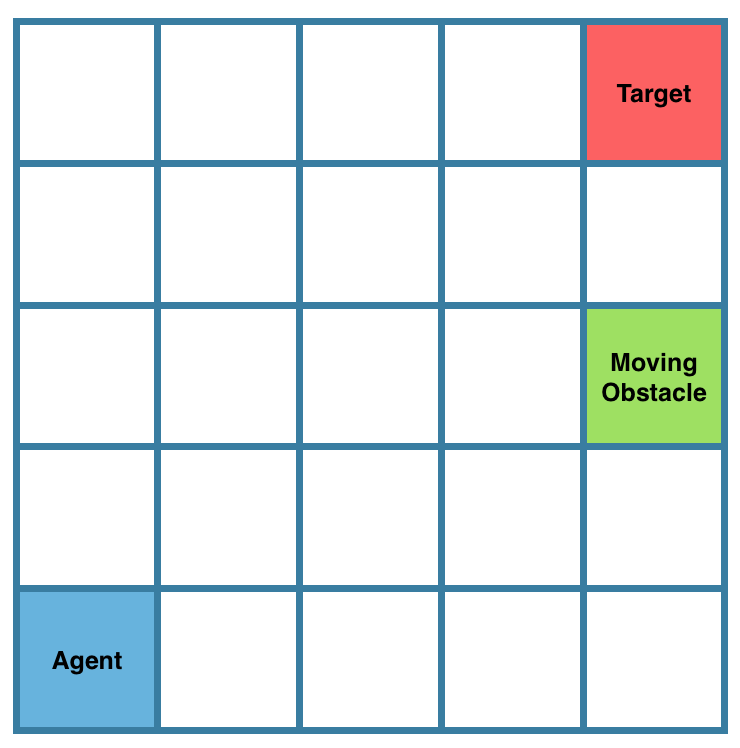
\includegraphics[width=0.4\textwidth]{figures/gridworld.png}
%\vspace{-4mm}
  \caption{Simulated social navigation task.} \label{fig:gridworld}
\end{figure}

% \begin{figure}[t]
%   \centering
%   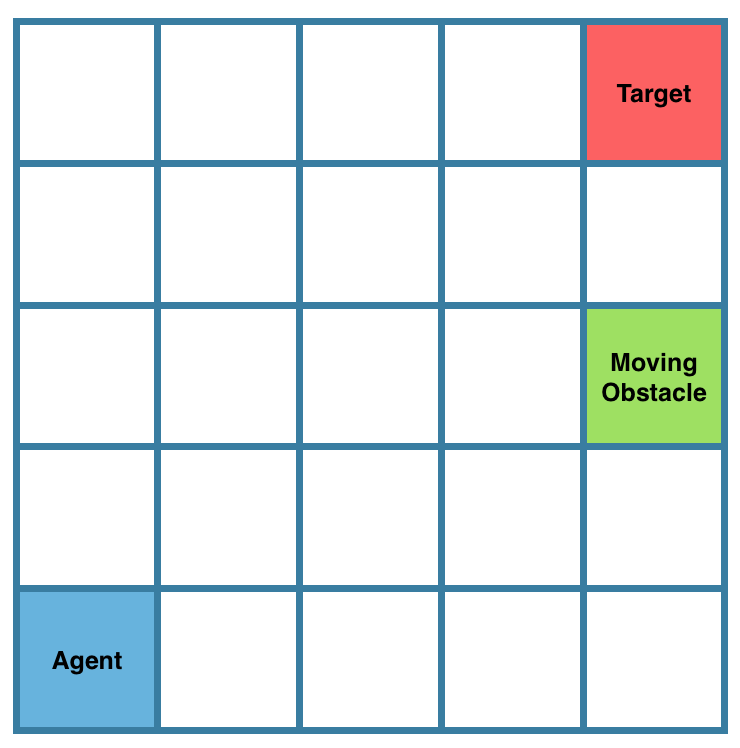
\includegraphics[bb=0 0 533 539,width=0.5\columnwidth]{figures/gridworld.png}
%   \caption{Moving obstacle gridworld 	\label{fig:gridworld}}
% \end{figure}
We first manually define two ground truth reward functions, $R^{\mathcal{D}^*} = w^{\mathcal{D}^*}\phi(s,a)$, $R^{\mathcal{F}^*} = w^{\mathcal{F}^*}\phi(s,a)$, described further below. Then, we sample initial test states from a uniform distribution over the state space, over which we define $P^{s_1}_{test}$, for all experimental runs. These initial conditions, along with the optimal maximum-entropy policies for $R^{\mathcal{D}^*}$ and $R^{\mathcal{F}^*}$, allow us to compute feature expectations $\widetilde{\mu}^{\mathcal{D}_{test}}$ and $\widetilde{\mu}^{\mathcal{F}_{test}}$ respectively. For each experimental run, we then sample a set of initial training states, over which we define $P^{s_{1}}_{train}$, %\jm{this is another prior distribution, not a set of states}
and generate the respective feature expectations $\widetilde{\mu}^{\mathcal{D}_{train}}$, $\widetilde{\mu}^{\mathcal{F}_{train}}$. These feature expectations are used to learn reward functions and their corresponding  policies using each algorithm under evaluation. Each learned policy $\pi^*$ is then executed from initial states sampled from $P^{s_{1}}_{test}$ to determine $\mu^{\pi^*}|_{test}$, the feature expectations for the policy at those initial conditions. Finally, we compute the values of each policy, at those initial conditions, with respect to the two reward functions, $V^{\pi^*}_{\mathcal{D},test} = (w^{\mathcal{D}^*})^T\mu^{\pi^*}|_{test}$, $V^{\pi^*}_{\mathcal{F},test} = (w^{\mathcal{F}^*})^T\mu^{\pi^*}|_{test}$. A good algorithm will yield a high $V^{\pi^*}_{\mathcal{D},test}$ and a low $V^{\pi^*}_{\mathcal{F},test}$ .

\begin{figure*}[h!]
  \centering
  \begin{subfigure}[t]{0.49\columnwidth}
    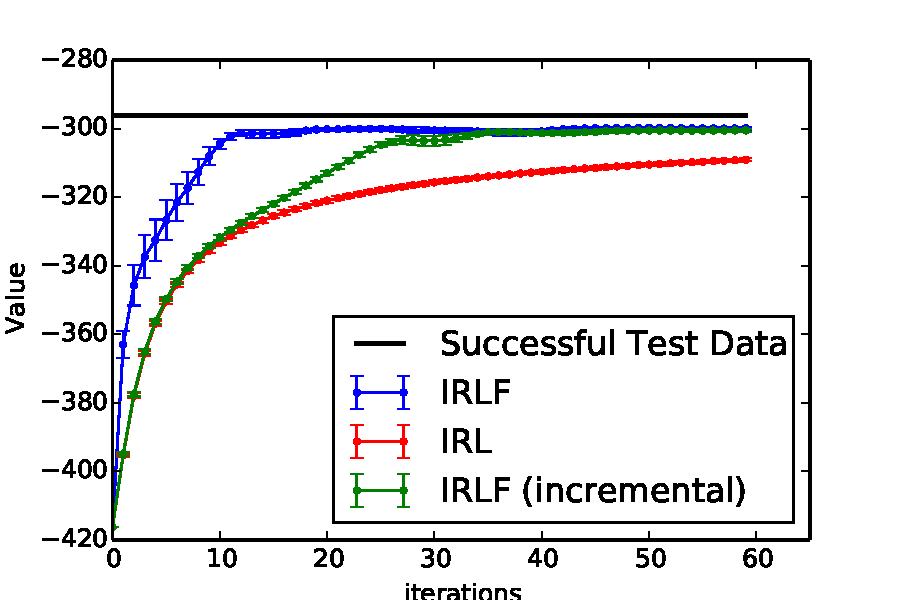
\includegraphics[clip=true,width=1.0\textwidth]{figures/expert_apprentice_contrastive.pdf}
    \caption{Contrasting w.r.t.\ $w^{\mathcal{D}^*}$}
    \label{fig:toy_expert_apprentice_contrastive}
   \end{subfigure}
     \begin{subfigure}[t]{0.49\columnwidth}
    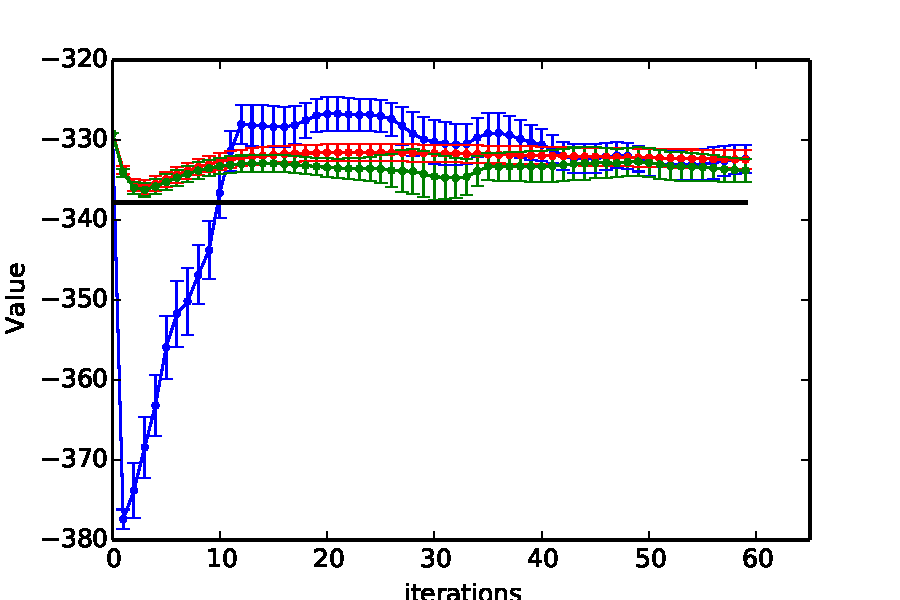
\includegraphics[clip=true,width=1.0\textwidth]{figures/taboo_apprentice_contrastive.pdf}
    \caption{Contrasting w.r.t. $w^{\mathcal{F}^*}$}
    \label{fig:toy_taboo_apprentice_contrastive}
   \end{subfigure}
   \\
   \begin{subfigure}[t]{0.49\columnwidth}
   \hspace{2mm}
    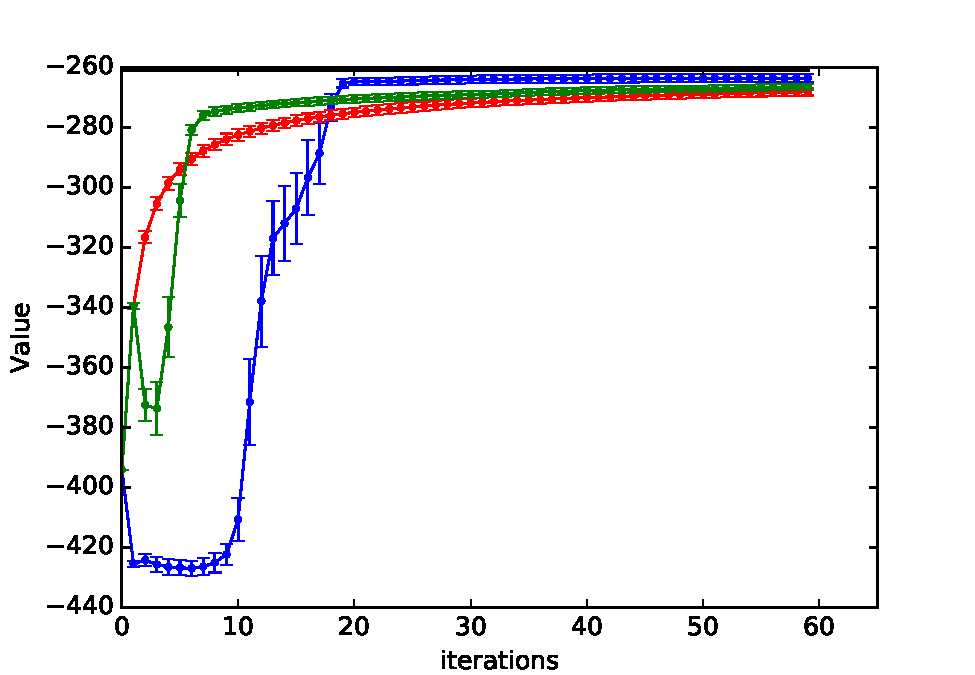
\includegraphics[trim=0.6cm 0.0cm 0.0cm 0.0cm,clip=true,width=0.95\textwidth]{figures/over_expert_apprentice.pdf}
    \caption{Overlapping w.r.t.\ $w^{\mathcal{D}^*}$}
    \label{fig:toy_expert_apprentice_overlapping}
    \end{subfigure}
   \begin{subfigure}[t]{0.49\columnwidth}
   \hspace{2mm}
    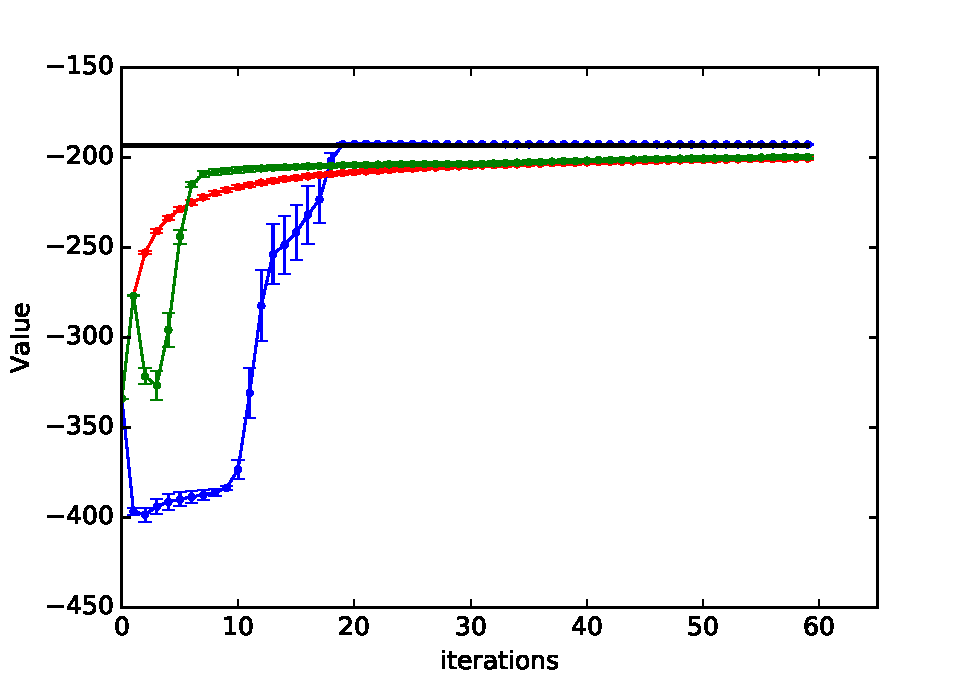
\includegraphics[trim=0.6cm 0.0cm 0.0cm 0.0cm,clip=true,width=0.95\textwidth]{figures/over_taboo_apprentice.pdf}
    \caption{Overlapping w.r.t.\ $w^{\mathcal{F}^*}$}
    \label{fig:toy_taboo_apprentice_overlapping}
    \end{subfigure}
    \\
    \begin{subfigure}[t]{0.49\columnwidth}
   \hspace{2mm}
    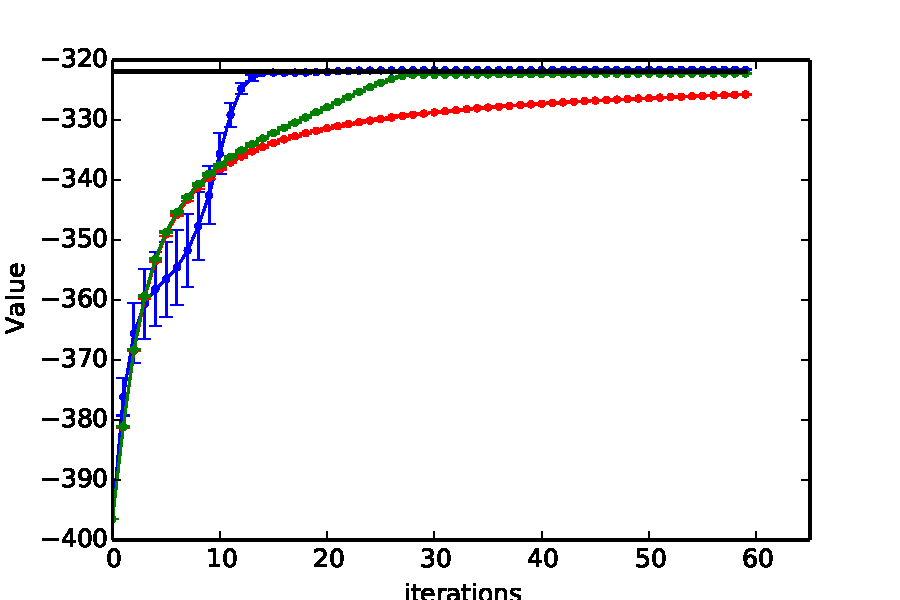
\includegraphics[trim=0.6cm 0.0cm 0.0cm 0.0cm,clip=true,width=0.95\textwidth]{figures/expert_apprentice_complementary.pdf}
    \caption{Complementary w.r.t.\ $w^{\mathcal{D}^*}$}
    \label{fig:toy_expert_apprentice_complementary}
    \end{subfigure}
    \begin{subfigure}[t]{0.49\columnwidth}
       \hspace{2mm}
    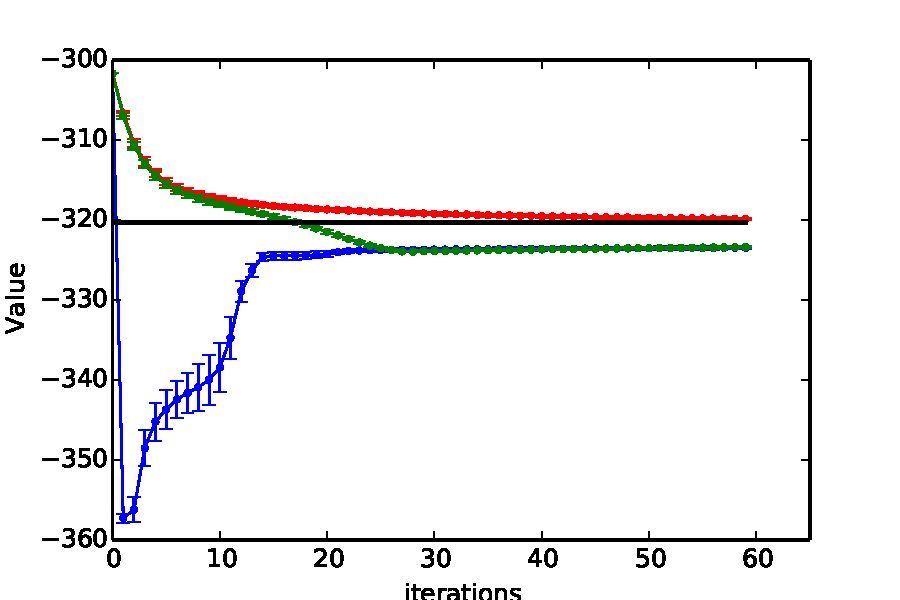
\includegraphics[trim=0.6cm 0.0cm 0.0cm 0.0cm,clip=true,width=0.95\textwidth]{figures/taboo_apprentice_complementary.pdf}
     \caption{Complementary w.r.t.\ $w^{\mathcal{F}^*}$}
    \label{fig:toy_taboo_apprentice_complementary}
    \end{subfigure}
    % 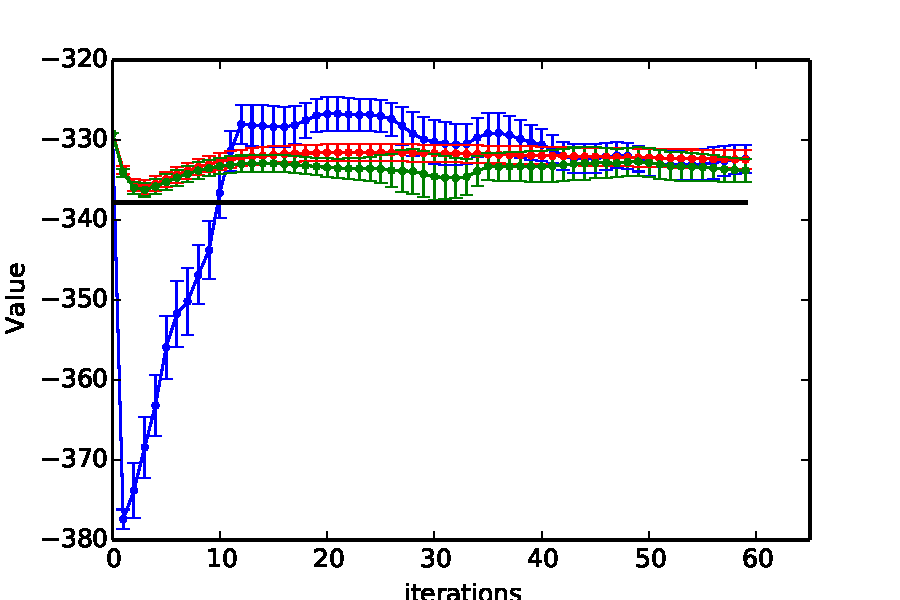
\includegraphics[clip=true,width=0.32\textwidth]{figures/taboo_apprentice_contrastive.pdf}
    % 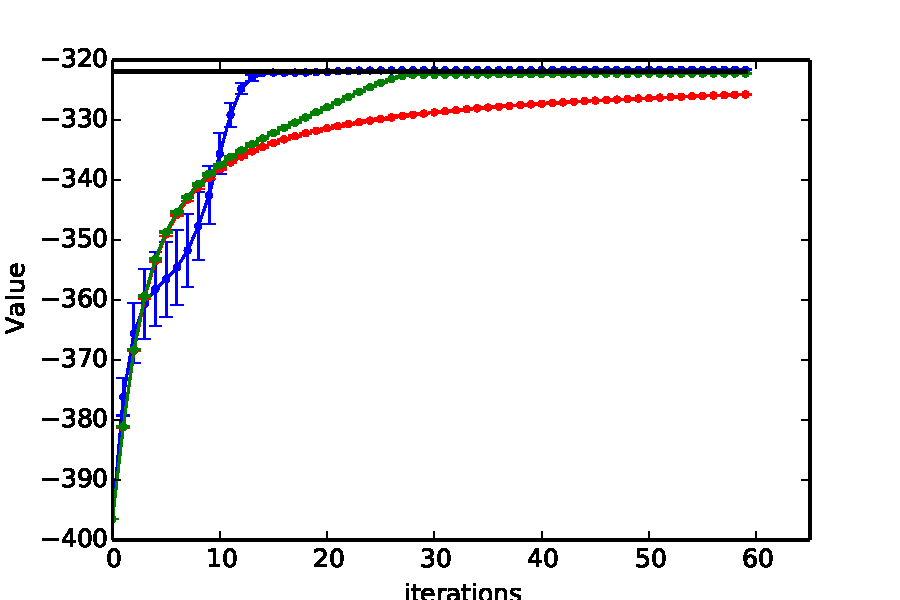
\includegraphics[clip=true,width=0.32\textwidth]{figures/expert_apprentice_complementary.pdf}
    % 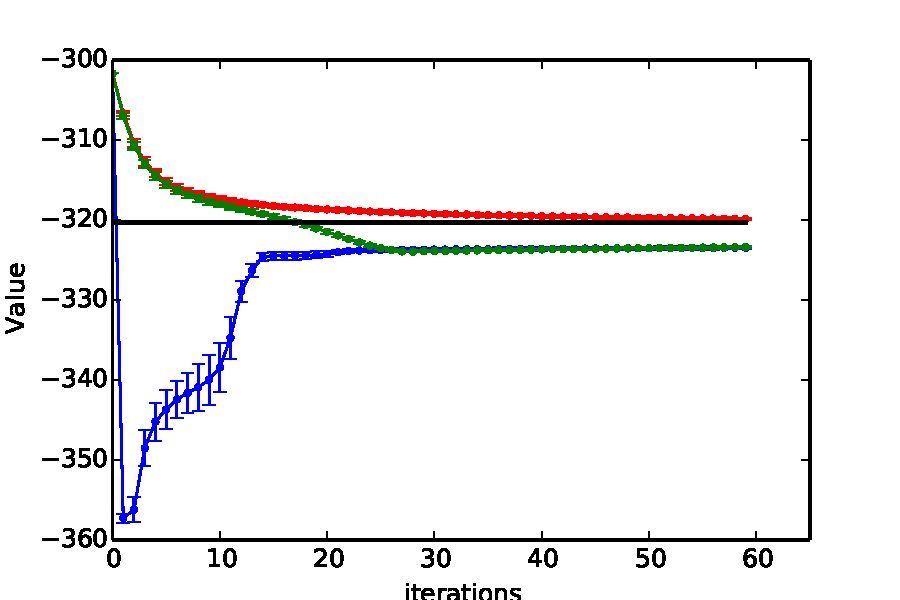
\includegraphics[clip=true,width=0.32\textwidth]{figures/taboo_apprentice_complementary.pdf}
  \caption[Value over 60 iterations.]{Value over 60 iterations, for 20 runs in contrasting, complementary and overlapping simulated domains w.r.t. $w^{\mathcal{D}^*}$ and $w^{\mathcal{F}^*}$.}
  %\vspace{-3mm}
  \label{fig:complementary}

\end{figure*}

% The learner has access to two sets of trajectories, $\mathcal{D}_{train},\mathcal{F}_{train}$, of length $h = 15$. The trajectories in $\mathcal{D}_{train}$ are generated using a reward function $R^\mathcal{D} = w^\mathcal{D}\phi(s,a)$ and summarised by their feature expectations $\widetilde{\mu}^{\mathcal{D}_{train}}$. Likewise the tranjectories in $\mathcal{F}_{train}$ are generated by a reward function $R^\mathcal{F} = w^\mathcal{F}\phi(s,a)$ and summarised by $\widetilde{\mu}^{\mathcal{F}_{train}}$. The underlying ``true'' reward functions $R^\mathcal{D}$ and $R^\mathcal{F}$ represent, respectively, the positive aspects of the domains such as reaching the target, and its negative aspects such as hitting the obstacle. The reward functions are not known to the learner. \jm{need more detail on the reward function. What are the specific numbers for these things? Otherwise, we need to make the code available and link it, for this to be reproducible.}

% Two more sets of trajectories, namely $\mathcal{D}_{test}$ and $ \mathcal{F}_{test}$, are used to assess the learner's performance on the task. The evaluation takes place by measuring the value accumulated by the agent based on the respective dataset's true reward function. Using equation \eqref{eq:parametrized_value} this is simply,
% \begin{align}
% &V^{\pi}_{\mathcal{D}} = (w^\mathcal{D})^T\mu^\pi|_\mathcal{D}\\
% &V^{\pi}_{\mathcal{F}} = (w^\mathcal{F})^T\mu^\pi|_\mathcal{F}. \label{eq:value_on_expert}
% \end{align}
% In other words, we can use the weights for each of the reward functions, along with the feature expectations associated with the execution of a policy from a certain set of initial conditions, to measure the performance of the agent with respect to that reward function. If therefore follows that a well-performing algorithm will maximise $V^{\pi}_{\mathcal{D}_{test}}$ and minimise $V^{\pi}_{\mathcal{F}_{test}}$. 

% In our experiments we fix $10$ test states (and their respective feature expectations) and perform experimental runs, for which we train our IRLF algorithm and its original counterpart, the MaxCausEnt IRL algorithm, on randomised initial conditions. The performance of the learned reward functions (and policies) at the fixed initial test states is evaluated using \eqref{eq:value_on_expert}. \jm{this sentence doesnt make sense.}\ks{I wanted to say that we learn on some initial conditons and test on others.}

Within this domain, we consider three scenarios that differ in how $R^{\mathcal{D}^*}$ and $R^{\mathcal{F}^*}$ are defined.  In the \emph{contrasting scenario}, $w^{\mathcal{D}^*}$ rewards reaching the target and avoiding the obstacle, while $w^{\mathcal{F}^*}$ rewards being in the same cell as the obstacle.  This scenario examines the value of completely failed demonstrations when the successful demonstrations already show the complete desired behaviour. 

In the \emph{overlapping scenario}, $w^{\mathcal{D}^*}$ is as before but $w^{\mathcal{F}^*}$ rewards not only colliding with the obstacle, but also reaching the target. This scenario examines the value of failed demonstrations when they are similar in some respects to the successful demonstrations. 

In the \emph{complementary scenario}, $w^{\mathcal{D}^*}$ rewards only reaching the target, while $w^{\mathcal{F}^*}$ only rewards hitting the obstacle. This scenario examines the value of failed demonstrations when the successful demonstrations do not fully disambiguate the desired behaviour.

Figures \ref{fig:toy_expert_apprentice_contrastive} and \ref{fig:toy_taboo_apprentice_contrastive} compare the performance of IRLF, with and without incremental updates to $\lambda$, to that of IRL in the contrasting scenario. Both versions of IRLF successfully utilise failed demonstrations to learn better and faster than IRL in terms of $V^{\pi^*}_{\mathcal{D},test}$.  They achieve similar performance to IRL in terms of $V^{\pi^*}_{\mathcal{F},test}$.  

Figures \ref{fig:toy_expert_apprentice_overlapping} and \ref{fig:toy_taboo_apprentice_overlapping} show results for the overlapping scenario. Even in this challenging setting, IRLF learns better than IRL, demonstrating the resilience of our method to the fact that some successful and failed trajectories might be similar and showing that our method can exploit the additional data found in failed trajectories without negative side effects. 

Finally, Figures \ref{fig:toy_expert_apprentice_complementary} and \ref{fig:toy_taboo_apprentice_complementary} show similar results for the complementary scenario.  The IRLF methods again perform better in terms of $V^{\pi^*}_{\mathcal{D},test}$ but now also perform better in terms of $V^{\pi^*}_{\mathcal{F},test}$.  In fact, they outperform even the successful data in terms of $V^{\pi^*}_{\mathcal{F},test}$, a consequence of the complementary nature of the reward functions. 

IRLF's performance with respect to $V^{\pi^*}_{\mathcal{F},test}$ (Figure \ref{fig:complementary} bottom row) illustrates how the algorithm gives priority to successful demonstrations when necessary. For the contrasting scenario, the probability of approaching the obstacle is already low for $w^{\mathcal{D}^*}$; therefore, IRL and IRLF behave similarly with respect to $w^{\mathcal{F}^*}$. In the ovelapping scenario, IRLF gives priority to reaching the target quickly, since this matches the behaviour in the successful demonstrations (even though it is discouraged from doing so by the failed demonstrations). Doing so means accumulating more value in terms of $V^{\pi^*}_{\mathcal{F},test}$. In the complementary scenario, since it is possible to satisfy both objectives simultaneously (reaching the target and avoiding obstacles), IRLF finds a reward function that performs well with respect to the succesful demonstrations while at the same time having a lower value with respect to the failed demonstrations.

 In all scenarios, IRLF is more stable with incremental updates than without.  In the contrasting and complementary scenarios, IRLF with incremental updates learns more slowly, while in the overlapping scenario it learns faster initially but plateaus slightly lower.

 In the experiments above, all methods received successful and failed demonstrations from five initial states. Hence, the results do not address how the number of succesful demonstrations given to the two learners affects their performance on the test set. In the complementary scenario, failed demonstrations are obviously important regardless of how many succesful demonstrations are available. In the other scenarios, however, it is not clear whether failed demonstrations are still useful even when successful demonstrations are abundant.

To test this, we repeated our experiments in the constrasting scenario but with 5, 50, 200 and 2000 initial states for successful demonstrations, while keeping the failed demonstrations to 5. For each algorithm, we plot  $(w^{\mathcal{D}^*})^T\widetilde{\mu}^{\mathcal{D}_{test}}$ - $V^{\pi^*}_{\mathcal{D},test}$ after 60 iterations of the algorithm. The smaller this value, the closer the learner comes to replicating the expert on the test set of initial states. The results, shown in Figure \ref{fig:data_size}, demonstrate that IRLF maintains its superiority over IRL even if the number of initial states for which demonstrations are given rises significantly. 

\begin{figure}
	\centering
 	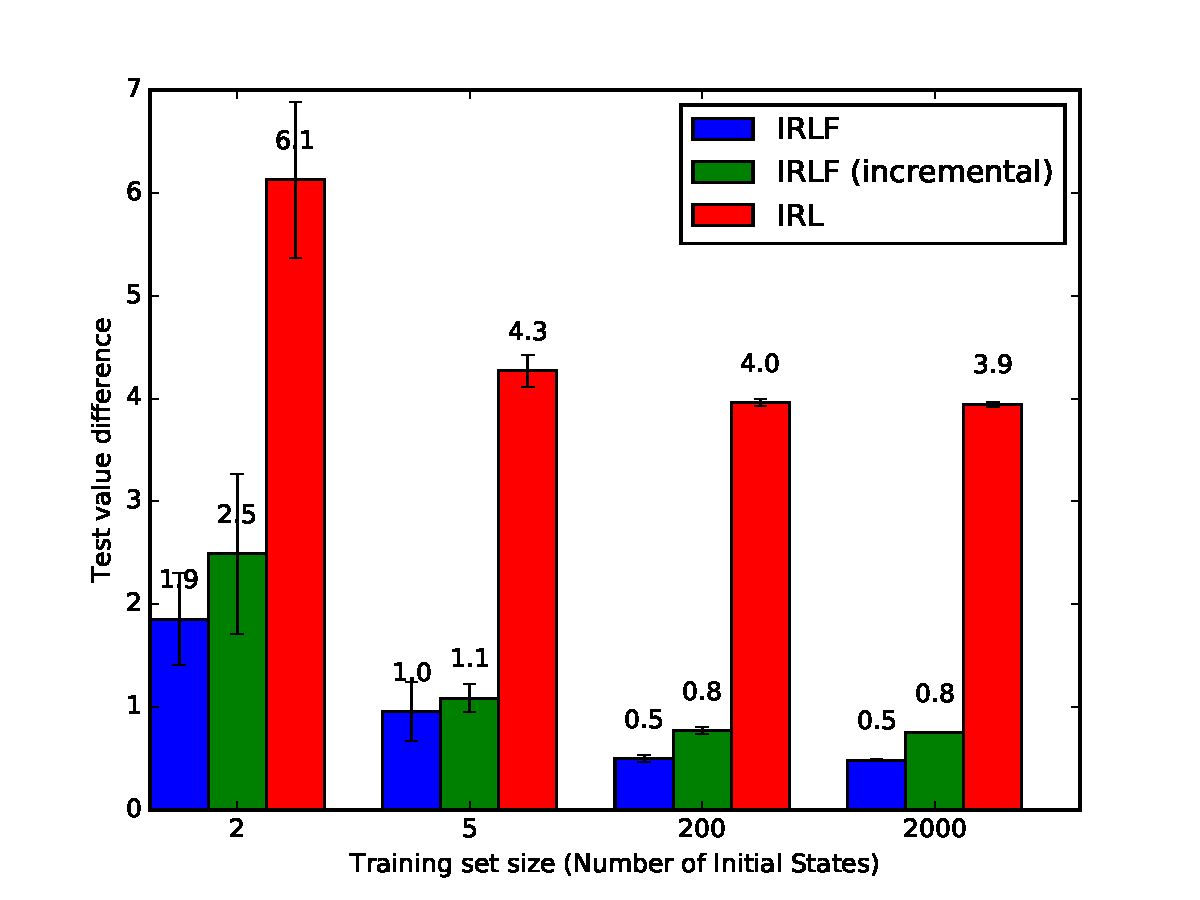
\includegraphics[clip=true,width=0.55\textwidth]{figures/data_size.pdf}
 	\caption[Performance of all three methods in the constrasting scenario.]{Performance of all three methods in the constrasting scenario for different numbers of initial states.}
 	\label{fig:data_size}
\end{figure}

To shed more light on IRLF's behaviour, Figure \ref{fig:rf_plot} plots the original and learned reward functions for IRL and IRLF for the contrasting scenario. In the original reward function $w^{\mathcal{D}^*}$ (Figure \ref{fig:rf_plot_good}), the obstacle is in cell [2,2] and the goal in cell [4,4], which explains the dips and spikes in those locations.  The reward function learned by IRL (Figure \ref{fig:rf_plot_irl}) is flat in the area of the obstacle. However, IRLF, by employing $w^{\mathcal{F}^*}$ (Figure \ref{fig:rf_plot_bad}) learns a reward function (\ref{fig:rf_plot_irlf}) that properly assigns a low reward to the obstacle and its surroundings. The reward function resulting from IRLF can therefore generalise better to unseen initial conditions and environments.


\begin{figure*}[thb]
  \centering
  \begin{subfigure}[b]{0.42\columnwidth}

    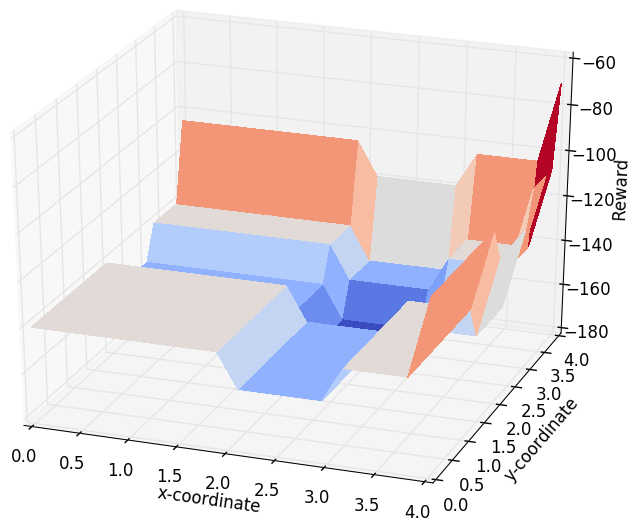
\includegraphics[clip=true,width=\textwidth]{figures/RF_D.png}

    
    \caption{\ $w^{\mathcal{D}^*}$}
    \label{fig:rf_plot_good}
  \end{subfigure}
  %\hfill
  \begin{subfigure}[b]{0.42\columnwidth}

    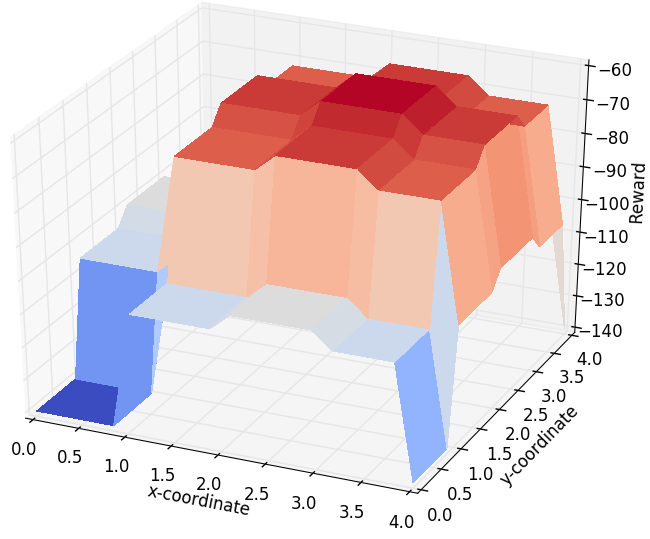
\includegraphics[clip=true,width=\textwidth]{figures/RF_F.png}

    
    \caption{\ $w^{\mathcal{F}^*}$}
    \label{fig:rf_plot_bad}
  \end{subfigure}  
  \\
  \label{fig:contrastive}
  \begin{subfigure}[b]{0.42\columnwidth}
    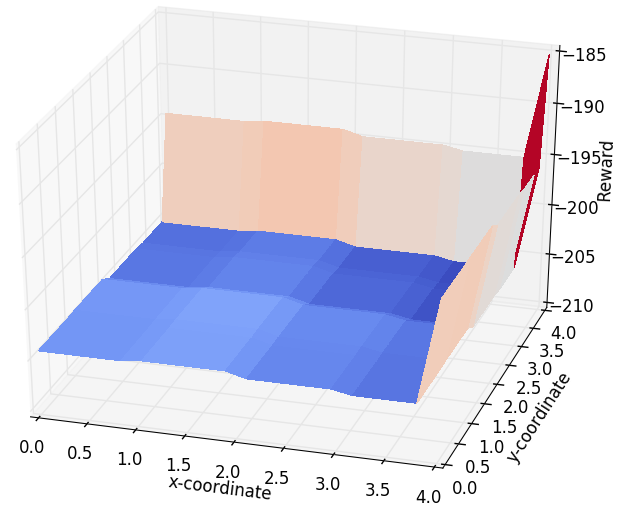
\includegraphics[clip=true,width=\textwidth]{figures/RF_IRL.png}
    \caption{IRL}
    \label{fig:rf_plot_irl}
  \end{subfigure}
  %\hfill
  \begin{subfigure}[b]{0.42\columnwidth}

    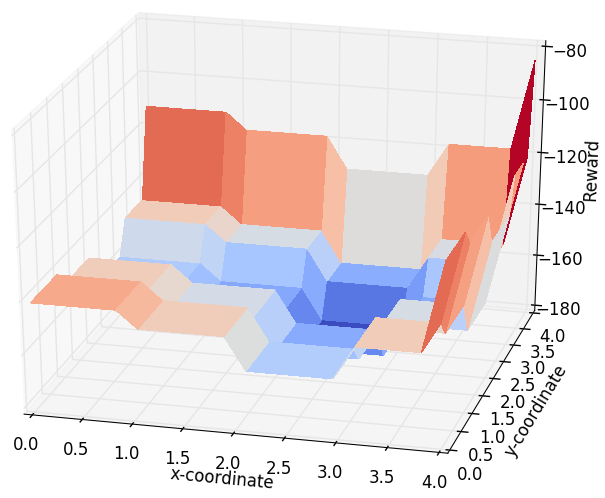
\includegraphics[clip=true,width=\textwidth]{figures/RF_IRLF.png}
    \caption{IRLF}
    \label{fig:rf_plot_irlf}
  \end{subfigure}  
  %\vspace{-3mm}
  \caption[The original reward and learned reward functions for the two algorithms.]{The original reward and learned reward functions for the two algorithms. Obstacle is static at [2,2]\ }
  %\vspace{-3mm}
  \label{fig:rf_plot}
\end{figure*}


% \begin{table}[]
% \centering

% \label{tab:results}
% \begin{tabular}{|l|l|l|l|}
% \hline
%            & $\theta_e(\Phi_{a}-\Phi_{e)}$& $\theta_t(\Phi_{a}-\Phi_{t)}$ & $|\pi_a - \pi_t|$ (\%) \\ \hline
% Original   & -6.125(2.06)        & 2.41(1.82)         & 15                    \\ \hline
% Our Method & 0(0.2)              & 0.02(0.167)        & 10                    \\ \hline
% \end{tabular}
% \caption{Results on test set after 20 runs of random initial conditions. $\theta_e$ represent reward weights, $\pi$ represents policy and $\Phi$ represents feature expectations. The subscripts $a,e,t$ represent the apprentice, expert and taboo agents respectively. \jm{This table needs to be cleaned up. Try to keep the same number of significant figures in all entries.}}
% \end{table}
% REAL DATA SECTION %

\subsubsection{Simulated Factory Domain}
Our second simulated domain is the \emph{Factory} benchmark problem proposed by Dearden \& Boutilier \cite{dearden1997abstraction}. In this domain, an autonomous agent is tasked with building an object according to specifications, which involves some sequence of shaping, painting, cleaning and assembly operations on its parts. Each individual operation costs some time and may have a probabilistic outcome, possibly resulting in unwanted side effects on the condition of each of the parts. Furthermore, there are precedence conditions on some of these operations -- for instance, parts must be shaped before they can be assembled. The goal of this domain is to produce the object in the most cost-efficient way.

While this problem has been previously tackled from the perspective of off-line decision-theoretic planning, it is a suitable domain to demonstrate the applicability of learning from demonstration, and in particular of IRLF. In a real manufacturing problem, human demonstrations on how to properly execute the manufacturing task, as well as failed demonstrations, in which the resulting object did not meet the quality specifications, would be readily available. Furthermore, consider a situation where the conditions in the factory problem may be subject to changes (for example, in the shapes or sizes of the parts) which may affect the optimal manufacturing policy. Learning a reward function, as opposed to learning a policy from demonstration, would make it easier for an autonomous agent to adapt to these changes.

\begin{figure}[tbh]
	\centering
%	\hspace{-5cm}
      \begin{subfigure}[b]{0.4\columnwidth}
      \hspace{-11mm}
    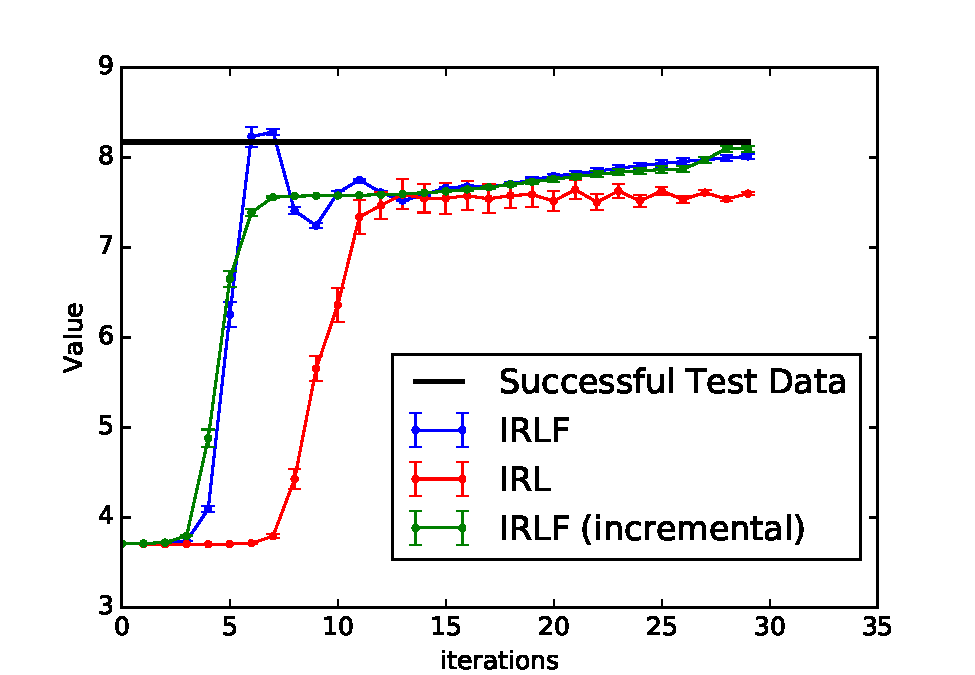
\includegraphics[clip=true,width=1.25\textwidth]{figures/factory_1.pdf}
    \caption{Value w.r.t.\ $w^{\mathcal{D}^*}$}
    \label{fig:factory_1}
  \end{subfigure}
 % \hspace{5mm}
  \begin{subfigure}[b]{0.4\columnwidth}
    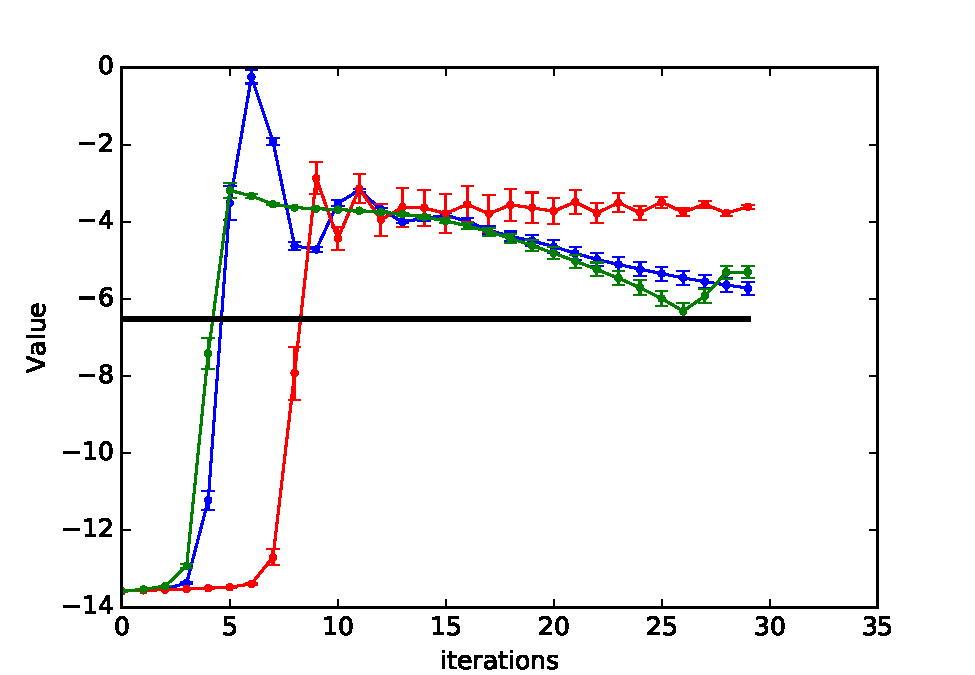
\includegraphics[trim=0.8cm 0.0cm 0.0cm 0.0cm,clip=true,width=1.20\textwidth]{figures/factory_2.pdf}
    \caption{Value w.r.t.\ $w^{\mathcal{F}^*}$}
    \label{fig:factory_2}
  \end{subfigure} 

  %\vspace{-3mm}
  \caption{Value over 30 iterations, for 15 runs of learning in the Factory domain.}
  %\vspace{-3mm}
  \label{fig:factory_results}

\end{figure}

Our instantiation of the Factory problem follows Dearden \& Boutilier's description \cite{dearden1997abstraction} (\emph{c.f.} Section A.2). It has $512$ states, factored into $9$ binary variables, and $10$ actions. The expert demonstrations were drawn from the optimal policy for that domain according to its original additive rewards ($w^{\mathcal{D}^*}_i$, Table \ref{tab:factory_reward}), while the failed demonstrations were drawn from a policy derived from a different reward function ($w^{\mathcal{F}^*}_i$, Table \ref{tab:factory_reward}). Note that we consider only $5$ features, corresponding to those state factors that have non-zero rewards. Each demonstration starts from random initial conditions and the evaluation proceeds in an identical manner to Section \ref{sec:sim_nav}.

\begin{table}[]
\centering

\begin{tabular}{|c|c|c|c|}
\hline
\begin{tabular}[c]{@{}c@{}}Feature\\Index $i$\end{tabular} & Proposition & $w^{\mathcal{D}^*}_i$ & $w^{\mathcal{F}^*}_i$\\ \hline
1                                                         & AClean      & 0.1 & 1    \\ \hline
2                                                         & BClean      & 0.1 & -0.1    \\ \hline
3                                                         & APainted    & 0.2 & 0.4    \\ \hline
4                                                         & BPainted    & 0.2 & 0    \\ \hline
5                                                         & Joined      & 0.4 & -2    \\ \hline
\end{tabular}
\caption{Reward functions for the Factory domain.\label{tab:factory_reward}}
\end{table}

% \begin{figure}[htb]     
%   \centering
%     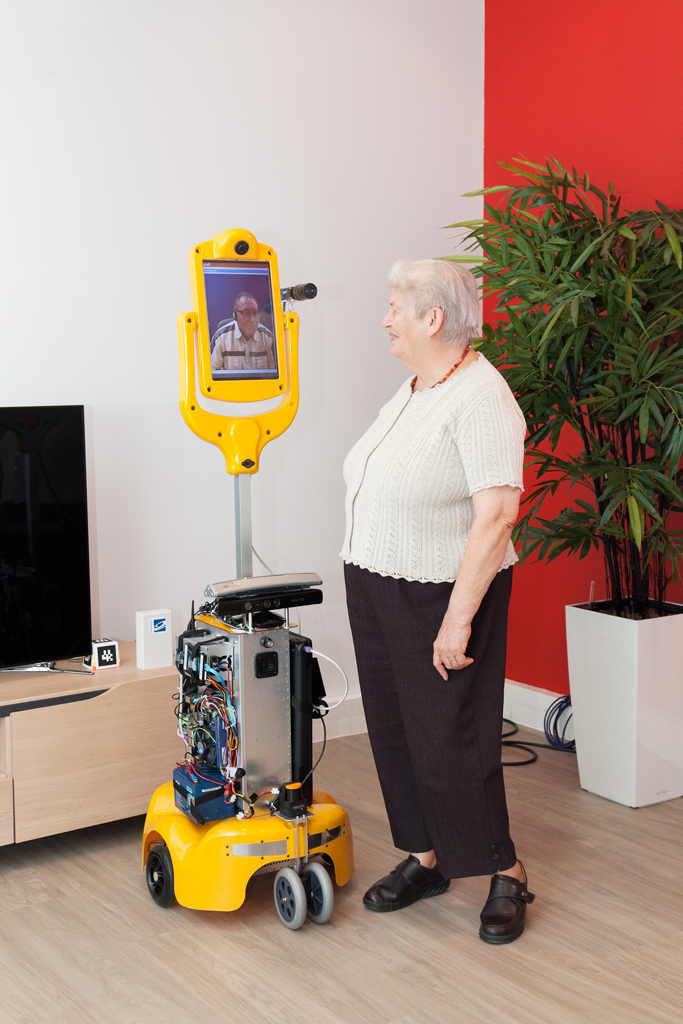
\includegraphics[width=0.75\columnwidth]{figures/robot.jpg}
%   \caption{The semi-autonomous telepresence robot used in our experiments.}
%   \label{fig:teresa_subject}
% \end{figure}

Figure \ref{fig:factory_results} shows the results, which are consistent with our previous observations. Figure \ref{fig:factory_1} shows that the reward function learned using IRLF is capable of yielding a policy that achieves a higher $V^{\pi^*}_{\mathcal{D},test}$ than IRL, and very close to that of the original policy. Furthermore, Figure \ref{fig:factory_2} shows that IRLF is capable of achieving lower $V^{\pi^*}_{\mathcal{F},test}$ than IRL. These results not only demonstrate the stability and reliability of IRLF, but further confirm the usefulness of failed demonstrations in inverse reinforcement learning.


\subsubsection{Real Navigation Domain}

We also evaluate the performance of IRLF on the social navigation dataset gathered in collaboration with UPO in Seville, and described in Section 4 of Deliverable 5.1 \cite{d5.1}. The collected dataset consists of 47 trajectories of an expert navigating the robot towards an interaction target while avoiding a moving or standing  person in a socially appropriate way. The positions of the people and the robot were accurately recorded using a motion capture system covering an area of $5m \times 5m$. A sample of the collected trajectories is shown in Figure \ref{fig:data}. 

For safety reasons, the failed dataset $\mathcal{F}$, which consists of $59$ trajectories, was collected by driving the robot in a simulator in a way that intentionally violates social norms, e.g., running into, following, or standing next to people. 

%\vspace{1mm}
\begin{figure}[t]     
%  \vspace{-2mm}
  \centering
    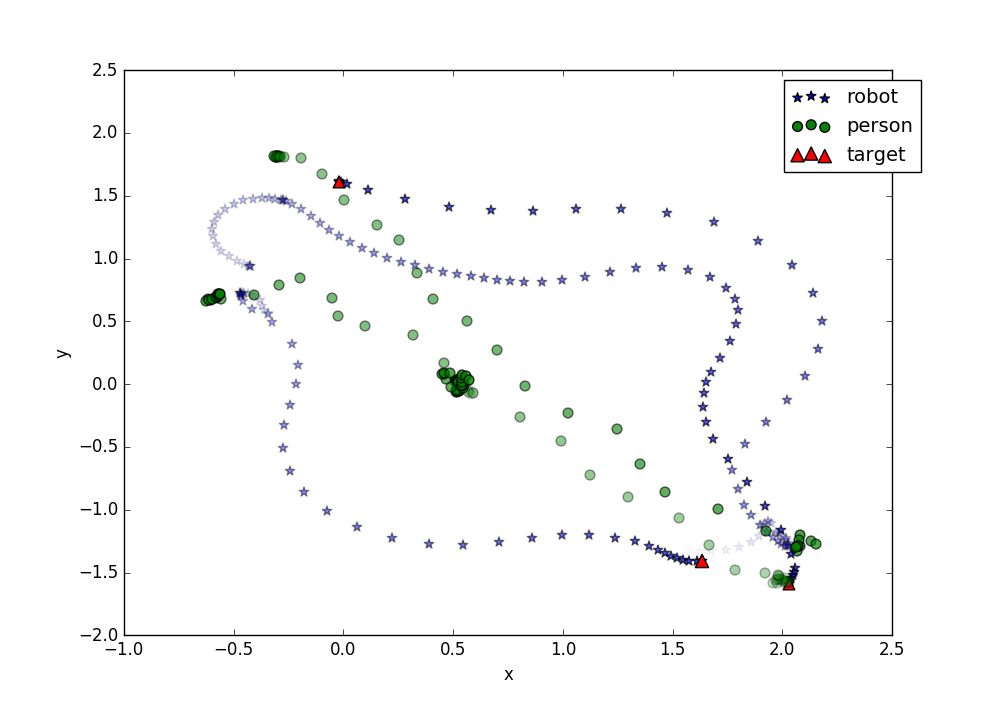
\includegraphics[width=0.55\columnwidth]{figures/data_plot.png}
  \caption[A sample of trajectories gathered using the TERESA robot.]{A sample of trajectories gathered using the TERESA robot. Darker dots occur later in time.}
  \label{fig:data}
\end{figure}

To model this domain as an MDP, we define a state space $S$ consisting of discretised positions for both the obstacle and the robot, as well as the discretised orientation of the obstacle, yielding a total of $837,808$ states. The action space consists of eight possible directions for robot movement, and an action that stops the robot. Using $\mathcal{D}$, we learned a factored stochastic transition function $T$. Furthermore, we defined a feature set $\phi(s,a)$ of $1401$ binary features, encoding the relative position of the robot from both the target and the obstacle, as well as their relative orientations. 

Applying IRL and IRLF to this domain is straightforward.  However, measuring performance is not, because we do not have access to the ground truth reward function needed to compute a policy's value. In previous work on IRL, researchers have taken multiple approaches to evaluation.  Some have considered simulated domains \cite{levine2011nonlinear,syed2007game,rothkopf2011preference} as in our results above, where a ground truth reward function is available. Others have considered real-world data but relied on qualitative evaluation \cite{ratliff2006maximum}, domain-specific performance measures \cite{neu2009training} or ad-hoc performance measures \cite{vasquez2014inverse}.

Since none of these approaches is entirely satisfactory, we adopt a different approach. First, we apply IRL to both $\mathcal{D}$ and $\mathcal{F}$ and derive reward functions, $R^{\mathcal{D}}$ and $R^{\mathcal{F}}$ and their respective weights $w^{\mathcal{D}^*}$ and $w^{\mathcal{F}^*}$, which we thereafter treat as ground truth.
Because MDPs are generative models, we can use these two separate reward functions to generate data while preserving access to the ground-truth reward functions that are so essential to evaluation. We are therefore able to conduct an evaluation analogous to the done in the simulated navigation domain, with the key difference that the $w^{\mathcal{D}^*}$ and $w^{\mathcal{F}^*}$ are learned from real data. 

Figure \ref{fig:paths}, which shows example trajectories generated by these reward functions, confirms that $w^{\mathcal{D}^*}$ produces human-like trajectories, while $w^{\mathcal{F}^*}$ generates inappropriate beha\-viour. These two reward functions can therefore be considered to be two separate agents whose demonstrations IRLF uses in order to learn a single reward function in a principled manner.

Figure \ref{fig:real_data} shows the results of our experiments on the real data, averaged across 6 independent runs. These results de\-monstrate that both versions of IRLF substantially outperform IRL with respect to $w^{\mathcal{D}^*}$.  The performance of all methods is similar with respect to $w^{\mathcal{F}^*}$, which suggests that, in this domain, imitating good behaviour is sufficient to score very low with respect to $w^{\mathcal{F}^*}$.  IRLF without incremental updates to $\lambda$ clearly oscillates, as expected, but still converges, while IRLF with incremental updates is stable and achieves a higher value than IRL.
%
Overall, the consistency of these results with those of the simulated domain provides further confirmation that failed demonstrations are useful for IRL, allowing it to generalise better to new initial conditions.  Furthermore, IRLF is a useful method for exploiting this data.

\begin{figure}[htb]

%  hspace{-16pt}
	\centering
	\begin{subfigure}[b]{0.4\columnwidth}
    \hspace{-5mm}
    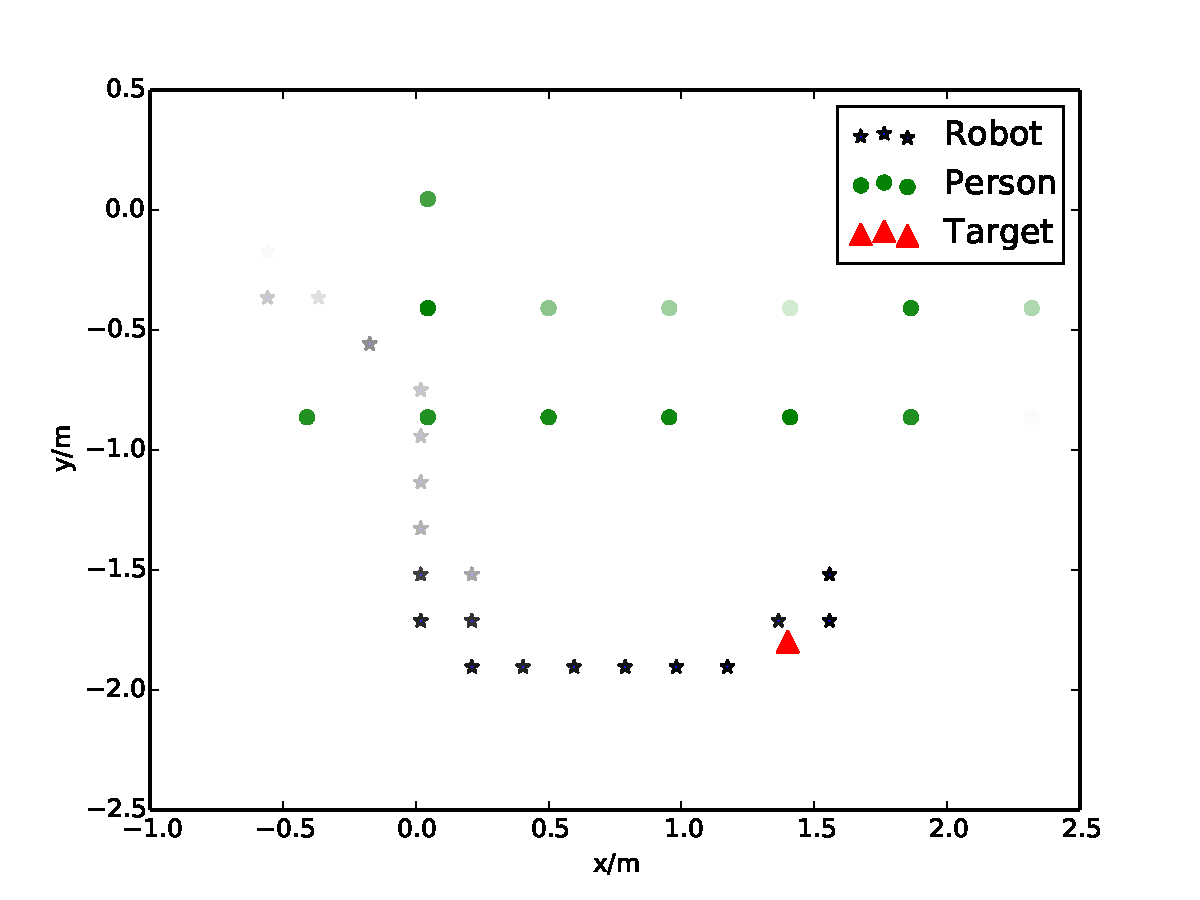
\includegraphics[scale = 0.35]{figures/gp.pdf}
    \end{subfigure}
    \begin{subfigure}[b]{0.4\columnwidth}
        \hspace{1mm}
    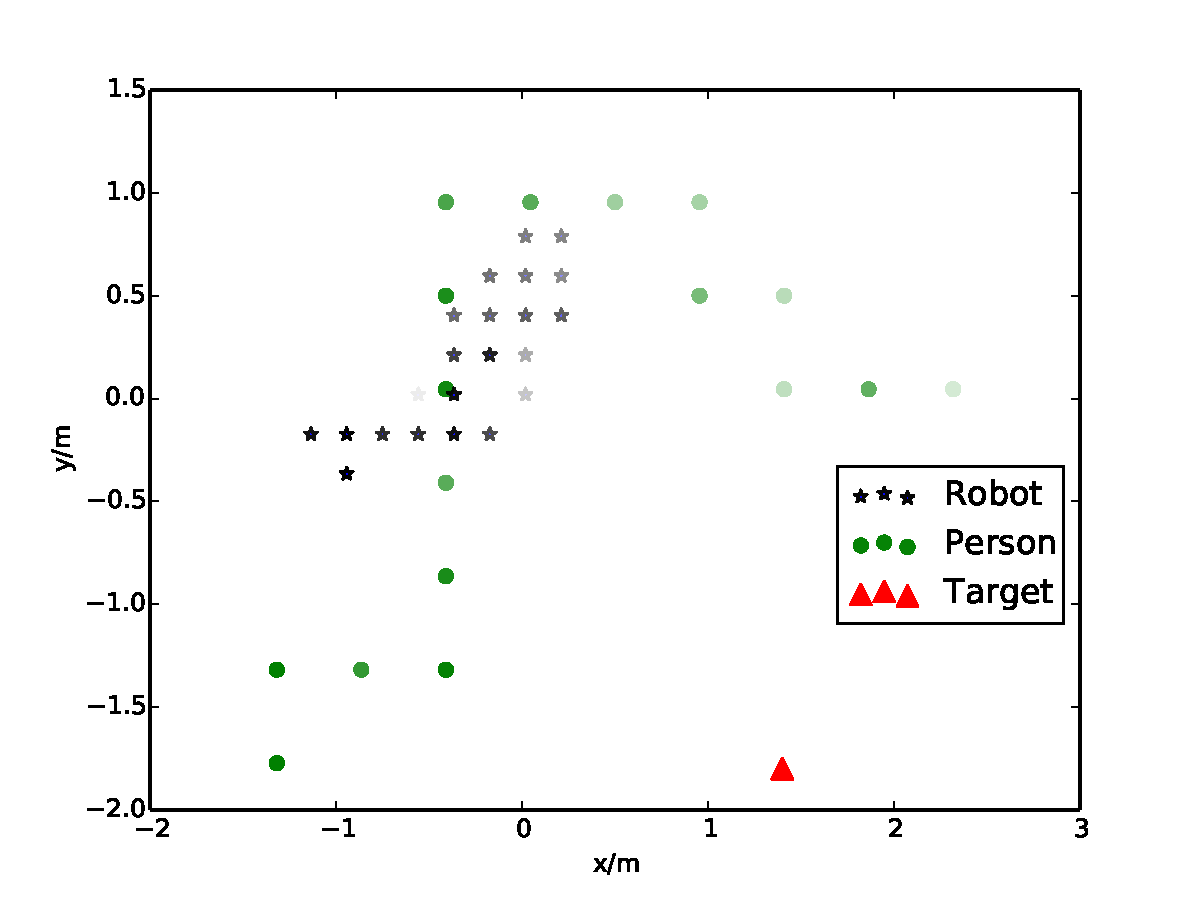
\includegraphics[scale = 0.35]{figures/bp.pdf}
  	\end{subfigure}
  \caption{Sample trajectories from $w^{\mathcal{D}^*}$ (left) and $w^{\mathcal{F}^*}$ (right). Darker dots occur later in time.} %These reward functions were learned from real data. The alpha channel denotes time}}
  \label{fig:paths}
\end{figure}


\begin{figure}[h!]
	\centering
	\begin{subfigure}[b]{0.4\columnwidth}
    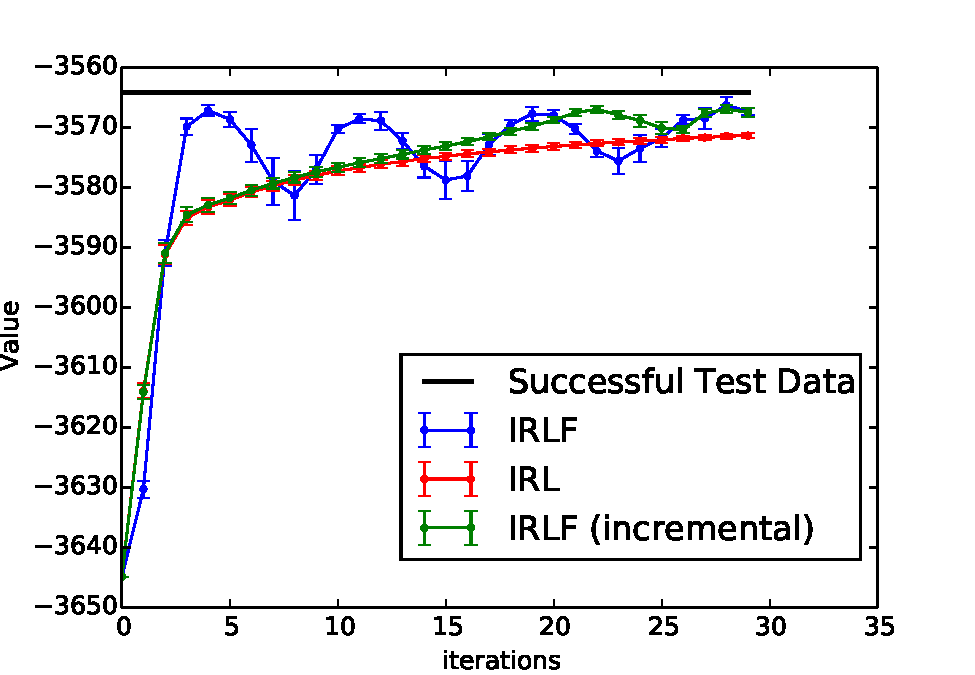
\includegraphics[trim=0.5cm 0.5cm 0.2cm 0.2,clip=true,width=1.1\textwidth]{figures/expert_apprentice_real.pdf}
    \caption{Value w.r.t.\ $w^{\mathcal{D}^*}$}
    \end{subfigure}
    \hspace{6mm}
    \begin{subfigure}[b]{0.4\columnwidth}
    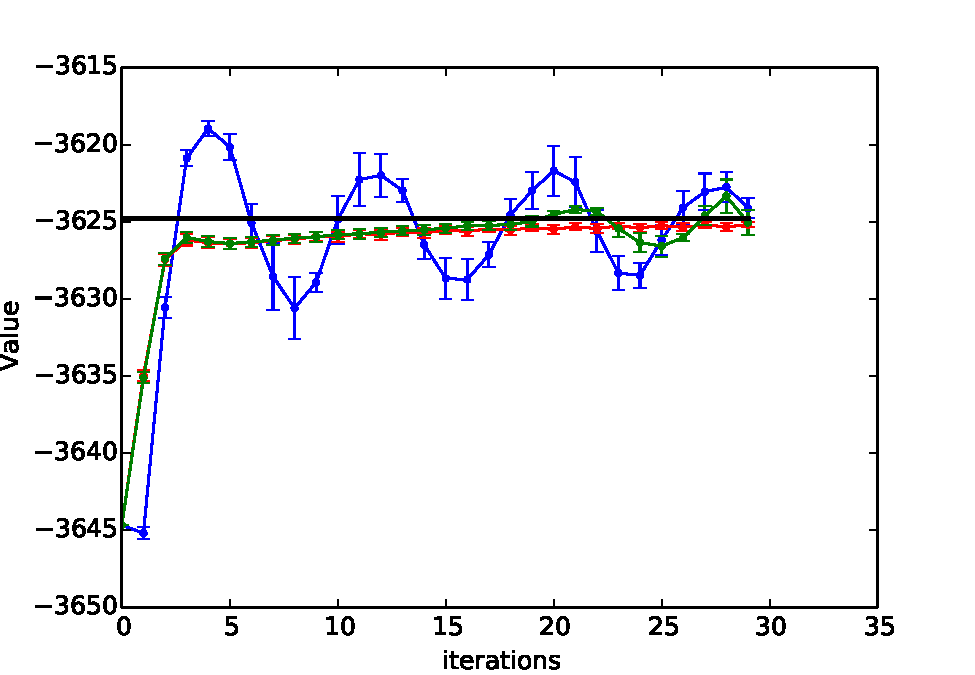
\includegraphics[trim=0.5cm 0.5cm 0.2cm 0.2,clip=true,width=1.1\textwidth]{figures/taboo_apprentice_real.pdf}
    \caption{Value w.r.t.\ $w^{\mathcal{F}^*}$}
  	\end{subfigure}
  \caption{Value over 30 iterations, for 6 runs on real data.}
  \label{fig:real_data}
  \vspace{-2mm}
\end{figure}


\subsection{Conclusions and Future Work}

% \sw{This can be modeled on the new abstract once it's written.  We do need some future work ideas.} \jm{Perhaps we can mention further robot tests and validation of these results as future work. There was also this idea on the table of coupling this learning from failure approach with other IRL / LfD algorithms}

This section introduced IRLF, the first inverse reinforcement learning algorithm that can learn from successful as well as failed demonstrations simultaneously. Starting from the maximum causal entropy IRL method, we proposed a new constrained optimisation formulation that accommodates both types of demonstrations and derived update rules for learning reward functions and policies. Our simulated navigation experiments investigated the properties of IRLF in cases where the succesful and failed demonstrations are either constrasting, overlapping, or complementary. The results in the overlapping scenario show that IRLF works even if the failed demonstrations are similar to the successful ones. We also presented results on a simulated factory domain as well as on real robot data from a social navigation task. These results clearly suggest that IRLF consistently learns faster and generalises better than the original IRL algorithm in consideration. In future work, we aim to investigate whether other IRL methods can also be extended to exploit failed demonstrations. In addition, we plan to conduct more experiments with real robots, including deploying an IRLF-learned policy on a robot. This will be facilitated using the RLT$^*$ method which is introduced in the next section.
\pagebreak


\section{Rapidly Exploring Learning Trees}
\label{sec:rrt-iros}
As we have seen in previous sections, IRL is a general method and can be used in conjunction with any decision-making task. When applied to robotics however, IRL falls under the more general umbrella term of learning from demonstration (LfD) \cite{argall2009survey}. LfD is of great interest to roboticists because it can avoid the need for tedious manual programming of complex behaviours. While most LfD methods rely on supervised learning to directly learn policies, certain approaches, such as IRL and the closely related field of inverse optimal control (IOC) \cite{kalman1964linear} instead learn \emph{cost functions} from demonstration. These cost functions are then used to \emph{plan} the robot's behaviour. 

Cost functions tend to be more general and robust to changes in the environment such as friction in a manipulator's joints. A robot trained in a supervised manner has less chance of adapting than one that has been trained using IRL or IOC because the cost function remains unchanged. In addition, cost functions are thought to be more succinct representations of the aims of the agent \cite{abbeel2004apprenticeship}. %For example, an agent that whose aim is to get as fast as possible to a goal location. The policy for such an agent will be much harder to interpret when compared to its cost function. 

However, inverse methods also have practical limitations. IRL for example requires modeling the task as a Markov decision process (MDP), which is typically impractical in robotics, for several reasons.  Firstly, an MDP assumes full observability. Secondly, planning in an MDP, which IRL methods must do repeatedly, is costly, especially in continuous and high-dimensional domains. Finally, the lack of scalability and the assumption of full observability prohibit the natural modeling of important factors such as kinodynamic constraints. Applying IRL to the real setting of the TERESA robot, therefore requires the invention of new methods that are more applicaple to robotics. 

Several researchers have proposed replacing the planning step in IRL with more convienient planners, e.g., Maximum Margin Planning (MMP)~\cite{ratliff2006maximum} uses A$^*$ search for planning. This avoids the need to do all the planning in advance, as is typical when solving an MDP. It also avoids the need to model all aspects of the environment since the robot can quickly replan its trajectory to account for uncertainty. However, deterministic search methods such as A$^*$ require discretisation of the state space, and quickly run into scalability problems as the discretisation becomes finer. Furthermore, this discretisation again ignores kinodynamic constraints.

In path planning, Rapidly Exploring Random Trees (RRTs)~\cite{lavalle1998rapidly} are popular because they cope well with continuous and high-dimensional domains and can elegantly handle kinodynamic constraints. The RRT$^*$ algorithm \cite{karaman2011sampling}, which extends RRTs to incorporate a cost function, is especially effective. However, the cost functions used by RRT$^*$ are typically simple and hand-coded and, to our knowledge, no methods have been developed to learn RRT$^*$ cost functions from demonstrations.


In this section, we propose Rapidly Exploring Learning Trees (RLT), which learns RRT$^*$ cost functions from demonstration. Specifically we modify Maximum Margin Planning to use RRT$^*$ as a planner. Furthermore, we propose a caching scheme that greatly reduces the computational cost of this approach. RLT requires no additional planner assumptions other than those inherent in RRT$^*$, making it particularly easy to implement. 

We evaluate RLT on real and simulated data from a social navigation scenario. The results demonstrate that RLT achieves better performance at lower computational cost than methods that learn path planning cost functions for deterministic planners.

\subsection{Related Work}

Substantial research has applied IRL to robotics \cite{henry2010learning,abbeel2008apprenticeship,vasquez2014inverse}. Because of the need to model the environment as an MDP, researchers usually discretise the state-action space. This introduces several key limitations. First, the size of the state-action space encountered in robotics is often prohibitive for such models. Second, the specific kinodynamic constraints of the robot cannot be easily be expressed by such representations, as they introduce non-Markovian dynamics. 

% \ks{Depending on the state-action space discretisation, past actions can infuence how easy it is to move to any a subsequent state. However the transition function only considers only one action in the past, and it is therefore an expectation over possible past configurations. As a result it tends to give the wrong probability distribution over next states for the actual physical system. Do I have to explain this in detail? Maybe Joao has a citation from his research?}

To apply IRL to more realistic situations, researchers usually try to replace the MDP model while retaining the main idea behind IRL, i.e., learning the underlying cost function of a planner using data from demonstrations. Maximum Entropy IRL \cite{ziebart2010modelingthesis} works in domains with linear continuous dynamics with the optimal controller being a Linear-Quadratic Regulator. Since linear dynamics are hard to come by in robotics, \cite{2012-cioc} considers locally linear aproximations. These bring about locally consistent rewards and achieve good performance in a range of tasks that were previously too hard for MDPs. However, the optimisation of the cost function using such planners is not guaranteed to be optimal. As our method is based on an RRT$^*$ planner, it is asymptotically optimal.

Other approaches to the problem use hybrid planners. Inverse Optimal Heuristic Control \cite{ratliff2009inverse} models the long-term goals of the agent as a coarse state MDP, to ensure tractability, while using supervised learning to determine the local policy of the agent at each state. Graph-Based IOC \cite{byravan2015graph} uses discrete optimal control on a coarse graph and the actual path is executed using local trajectory optimisation techniques such as CHOMP \cite{ratliff2009chomp}, which would otherwise suffer from local minima. The method is effective in robotic manipulation tasks with many degrees of freedom.  However, these methods employ complex and domain-specific planning formulations that are not suitable for all robotics tasks. The method presented here employs widely used planners, making it versatile and easy to implement. 

Another more recent graph-based concept is that of Adaptive State Graphs \cite{okallearning}, which build a controller graph before doing any learning. This controller graph is akin to \emph{options} in semi-Markov decision processes, and allows for a more flexible representation of the state-action space. However, the controller used to learn the underlying cost function is not the same as the one used to execute the robot's behaviour. This can have an adverse effect since an implicit assumption of IRL is that the demonstration paths came from the same planner that we use during learning. This planner has specific representations, such as discretisation and parameters such as the discount factor. If these change, different policies arise. As a result a path that was optimal under a certain planner ceases to be optimal under another.

RLT$^*$ can also be viewed as a graph-based, or rather tree-based, approach. Instead of building a controller graph first and then using different controllers to optimise trajectories, RLT$^*$ builds a controller tree on the fly. RLT$^*$ however uses the exact same planner during learning and execution.


\subsection{Background}
We begin with background on path planning and inverse reinforcement learning for path planning.

\subsubsection{Path Planning \label{subsec:path_planning}}
Path planning occurs in a space $\mathcal{S}$ of possible configurations of the robot. A configuration $s \in \mathcal{S}$ is usually continuous, and often represents spatial quantities such as position and orientation. A path planner seeks an obstacle-free path $\zeta_{o,g} = (s_1,s_2,s_3$ $\ldots,s_{l_{\zeta}}) $ of length $l_{\zeta}$, from an initial configuration $o = s_1$ to a goal configuration  $g =s_{l_{\zeta}}$. When the initial and goal configurations are implied, we refer to a path as $\zeta$.

Because there could be several paths to the goal, path planners typically employ a \emph{cost functional}, $C(\zeta)$ often defined as the sum of the costs between two subsequent configurations in a path $c(s_i,s_j)$. The total cost $C(\zeta)$ is therefore the sum of the individual costs along the path, i.e.,
\begin{equation}
	C(\zeta) = \sum_{i=1}^{l_{\zeta}-1} c(s_i,s_{i+1}).
\end{equation}
This cost functional is similar to the one encountered in optimal control as well as to value functions used in reinforcement learning. Given the cost functional, the path planner seeks an optimal path $\zeta^*$, which satisfies,
\begin{equation}
 	\zeta^*_{o,g} = \argmin_{\zeta_{o,g} \in Z_{o,g}} C(\zeta), \label{eq:back_plan}
\end{equation}
where $Z_{o,g}$ is the set of all possible paths such that $s_1 = o, s_{l_\zeta} = g$.

Many path planning algorithms discretise $\mathcal{S}$ and use graph search algorithms like A$^*$ to find the optimal path. Under mild assumptions, these approaches are guaranteed to find the best path on the graph, but not in $\mathcal{S}$. However, they scale poorly in the size of $\mathcal{S}$, as larger and larger graphs are required. Furthermore, such methods do not address kinodynamic constraints, i.e., they assume that every configuration on the graph is accessible from a neighbouring one. 

These drawbacks motivate \emph{sample-based} path planning algorithms such as RRT$^*$. Instead of building a graph and then searching it, RRT$^*$ builds a tree on the fly and keeps track of the current best path. This tree can be grown in a way that respects kinodynamic constraints. Furthermore, a sampled-based approach can quickly find good, but not optimal, paths in large configuration spaces.

%  RRT$^*$ is also asymptotically optimal, i.e., it is guranteed to find an optimal path in $\mathcal{S}$ as the sampling time goes to infinity. Many variants of RRT$^*$ provide improved performance and faster convergence in practice by, for example, heuristically shriking the sampling space \cite{gammell2014informed}.

% The most significant difference between A$^*$ and RRT$^*$ is that while former is deterministic, the latter is probabilistic. It is important to understand how this distinction affects learning.

A$^*$ can solve \eqref{eq:back_plan} for a subset $\tilde{Z}_{o,g} \in  Z_{o,g}$ that is determined by its resolution (discretisation). RRT$^*$, for a given time budget $T$, also minimises a subset but in this case $\tilde{Z}_{o,g}$ is determined by the randomly sampled points. As $T \rightarrow \infty$, RRT$^*$ minimises over the entire $Z_{o,g}$, i.e., it is asymptotically optimal. In other words, the RRT$^*$ is asymptotically optimal as a function of sampling time and A$^*$ is asymptotically optimal as a function of resolution. %This distinction will become very important when we attempt to learn cost functions for these planners in the next section.

\subsubsection{IRL for Path Planning \label{subsec:inverse_problem}}
Path planning involves finding a (near) optimal path to the goal given a cost function. In the inverse problem, we are given example paths and must find the cost function for which these paths are (near) optimal.  The example paths comprise a dataset $\mathcal{D} = (\zeta^1_{o_1,g_1},\zeta^2_{o_2,g_2}...\zeta^D_{o_D,g_D})$ where $\zeta^i_{o_i,g_i}$ is an example path with initial and final configurations $o_i,g_i$ respectively. We assume the unknown cost function is of the form,
\begin{equation}
	c(s_i,s_j) = \mathbf{w}^T \mathbf{f}(s_i,s_j), \label{eq:inner_prod}
\end{equation}
where $\mathbf{f}(s_i,s_j)$ is a $K$-dimensional vector of features that encode different aspects of the configuration pair and $\mathbf{w}$ is a vector of unknown weights to be learned. Since $\mathbf{w}$ is independent of the configuration, we can express the total cost of the path in a parametric form:

\begin{equation}
	C(\zeta) = \mathbf{w}^T\sum_{i=0}^{l_{\zeta}-1} \mathbf{f}(s_i,s_{i+1}) := \mathbf{w}^T \mathbf{F}(\zeta),
\end{equation}
where $\mathbf{F}(\zeta)$ is the \emph{feature sum} of the path.

While many formulations of the inverse problem exist, the general idea is to find a weight vector that assigns less cost to the example paths than all other possible paths with the same initial and goal configuration.  This can be formalised by a set of inequality constraints:

\begin{equation}
	C(\zeta^i_{o_i,g_i}) \leq  C(\zeta) \quad \forall \zeta \in Z_{o_i,g_i}  \quad \forall i. \label{eq:const1}
\end{equation}
The constraint is an inequality because $Z_{o,g}$ contains only paths available to the planner and thus may not include the example path $\zeta^i_{o_i,g_i}$.
$Z_{o_i,g_i}$ can be large but if we have an optimisation procedure that solves \eqref{eq:back_plan}, it is enough to satisfy, 
\begin{equation}
	C(\zeta^i_{o_i,g_i}) \leq \min_{\zeta \in Z_{o_i,g_i}} C(\zeta) \quad \forall i, \label{eq:const}
\end{equation}

Ratliff et al.\ \cite{ratliff2006maximum} propose a maximum margin variant of \eqref{eq:const} by introducing a margin function $L_i(\zeta)$ that decreases the cost of the proposed path $\zeta$ if is dissimilar to $\zeta^i_{o_i,g_i}$. For example, $L_i(\zeta)$ could be $-1$ times the number of configurations in the demonstration path not visited by $\zeta$. The full optimisation formulation of Maximum Margin Planning is as follows.

\begin{equation}
	\argmin_{\mathbf{w},\tau} \frac{1}{2}||\mathbf{w}||^2 + \frac{\lambda}{D} \sum_i \tau_i \label{eq:mas_marg}
\end{equation}
\begin{equation}
	\text{s.t.} \quad C(\zeta^i_{o_i,g_i}) - \tau_i \leq \min_{\zeta \in Z_{o_i,g_i}} C(\zeta) + L_i(\zeta) \quad \forall i,
\end{equation}
where $\tau_i$ are slacks that can be used to relax the constraints. Rearranging the inequality in terms of the slacks we get:

\begin{equation}
	 \quad C(\zeta^i_{o_i,g_i}) - \min_{\zeta \in Z_{o_i,g_i}} C(\zeta) + L_i(\zeta)  \leq \tau_i  \quad \forall i.
\end{equation}
Consequently, the $\mathbf{w}$ minimising:
\begin{equation}
	\frac{1}{2}||\mathbf{w}||^2 + \frac{\lambda}{D} \sum_i \big( C(\zeta^i_{o_i,g_i}) - \min_{\zeta \in Z_{o_i,g_i}}\big(C(\zeta) + L_i(\zeta)\big) \big) \big. \label{eq:unconstrained}
\end{equation}
is equivalent to that which minimizes \eqref{eq:mas_marg}, i.e., the slacks are tight.
The minimum can be found by computing a subgradient and performing gradient descent on the above objective:
\begin{equation}
	\nabla_{\mathbf{w}} =\mathbf{w} +  \frac{\lambda}{D} \sum_{i=0}^D F(\zeta^i_{o_i,g_i}) - F(\tilde{\zeta}^*_{o_i,g_i}), \label{eq:update1}
\end{equation}
where,
\begin{equation}
	\tilde{\zeta}^*_{o_i,g_i} = \argmin_{\zeta \in Z_{o_i,g_i}} C(\zeta) + L_i(\zeta). \label{eq:augmented_max}
\end{equation}

The inverse problem can therefore be seen as an iterative procedure, that first solves \eqref{eq:augmented_max} in the inner loop while keeping the weights constant. Based on that solution, it updates the weights using \eqref{eq:update1} in the outer loop. The weights at convergence represent the cost function that is used to plan the future behaviour of the agent. In \cite{ratliff2006maximum}, A$^*$ search was used for planning in the inner loop, assuming that the domain contained acyclic positive costs. In this work, we make the same assumptions but develop methods that use RRT$^*$ for planning.

\subsection{Method}
	In this section, we propose Rapidly Exploring Learning Trees (RLT$^*$).  We first propose a generic extension to the maximum margin approach that we call Approximate Maximum Margin Planning.  We then show how an implementation of this approach with an RRT$^*$ planner and a novel caching scheme yields RLT$^*$.

	% \subsection{Feature Sums and Sampled Based Planners}
	% 	Feature sums, $F(\zeta)$, can be seen as the  `fingerprints' of paths, and their definition is of crucial importance in the inverse problem. When planning on a fixed graph, like in the case of MDPs or A$^*$ search, it is easy to define the feature sums as the \emph{edge} costs on the graph. Furthermore if planning in continous domains we may consider integrals along the path. In RRT's however the tree that is being built has neither a fixed structure, nor an analytical form. Thus, the first step towards learning RRT$^*$ cost functions from demonstration is to come up with a reasonable approximation of $F(\zeta)$ for a path. This approximation must be consistent with the definition of the cost for a configuration pair. One such definition for cost is as follows.
	% 	\begin{equation}
	% 		c(s_i,s_j) = \frac{c(s_i)+c(s_j)}{2}d_{s_i,s_j}
	% 	\end{equation}
	% 	Where $c(s_i)$ is a cost function defined over a single configuration and $d_{s_i,s_j}$ is a measure of distance between the two configurations. For example if we consider configurations to be points in Eucledian space then $d_{s_i,s_j}$ can be the eucledian distance. Noting that the costs and features are related by \eqref{eq:inner_prod} for a single feature $f_k$ we have,

	% 	\begin{equation}
	% 		f_k(s_i,s_j) = \frac{f(s_i)+f(s_j)}{2}d_{s_i,s_j}
	% 	\end{equation}
	% 	Following this definition feature sum calculation along a candidate path is trivial,
	% 	\begin{equation}
	% 		F(\zeta) = \sum_{i=0}^{\zeta_l-1} \frac{\mathbf{f}(s_i)+\mathbf{f}(s_{i+1})}{2}d_{s_i,s_{i+1}}
	% 	\end{equation}

\subsubsection{Approximate Maximum Margin Planning \label{subsec:ammp}}

		In Section \ref{subsec:inverse_problem}, we showed how the multiple constraints of \eqref{eq:const1} could be reduced to a single constraint for each demonstration in \eqref{eq:const}. However, given a finite time budget $T$, a sample-based planner like RRT$^*$ minimises, not over the full set of paths $Z_{o,g}$, but over a randomly sampled $\tilde{Z}_{o,g}$. Thus, we can modify \eqref{eq:const}, and demand that our cost function satisfies,
\begin{equation}
	C(\zeta^i_{o_i,g_i}) \leq \min_{\zeta_{o_i,g_i} \in \tilde{Z}_{o_i,g_i}} C(\zeta) \quad \forall i. \label{eq:const_rrt}
\end{equation}
	As the planning budget $T$ increases, the sample-based planner samples lower cost paths, making this inequality harder to satisfy. Assuming $\tilde{Z}_{o_i,g_i}$ is constant, we can rewrite \eqref{eq:unconstrained} as:

	\begin{equation} \frac{1}{2}||\mathbf{w}||^2 + \frac{\lambda}{D} \sum_i \big( C(\zeta^i_{o_i,g_i}) - \min_{\zeta \in \tilde{Z}_{o_i,g_i}}\big(C(\zeta) + L_i(\zeta)\big) \big). \label{eq:unconstrained_rrt}
	\end{equation}
	This gives rise to an approach we call Approximate Maximum Margin Planning (AMMP), which is similar  to the one described in Section \ref{subsec:inverse_problem}, with the crucial difference that the planning step is executed by a sample-based planner and not a deterministic one, like A$^*$. An important consequence is that $\tilde{Z}_{o_i,g_i}$ now changes every time we invoke the sample-based planner. As a result, AMMP can be thought of as a smart way of sampling the \emph{constraints} that we want our cost function to satisfy. 


\subsubsection{Rapidly Exploring Learning Trees \label{subsec:cached}}

A simple way to construct a concrete algorithm from AMMP is to use RRT$^*$ as the sample-based planner.  However, this results in a computationally expensive algorithm, which calls the planner $I\times|D|$ times over $I$ iterations given a dataset of size $|D|$.  Since planning is typically expensive, it is crucial to find a more efficient approach.

In this section, we propose Rapidly Exploring Learning Trees (RLT$^*$), which implements AMMP with an RRT$^*$ planner but uses a caching scheme to achieve computational efficiency.

Two of the most costly operations of RRT$^*$ are 1) finding the nearest neighbour to a newly sampled point and 2) finding the radius-neighbours of a newly created vertex in the tree \cite{karaman2011sampling}. However, a key observation is that neither of these procedures depend on the cost function used by the planner. Thus,  RRT$^*$ can be split in two independent steps. 

	The first step is described in Algorithm \ref{alg:rrt_cache}, which takes as input $p$, the number of points to randomly sample from free space; $s_{init}$, the initial point; and $\eta$, the steer step size. For each randomly sampled point $s_{rand}$, we find the nearest neighbour, $s_{nearest}$, from the set of points in the vertex set $V$. We then create a new configuration point $s_{new}$ by steering from $s_{nearest}$ to $s_{rand}$. Next, we query the radius neighbours of $s_{new}$ at a radius determined by  $\min\{\gamma_{RRT^*}(\frac{\log(|V|)}{|V|})^{\frac{1}{d}},\eta\}$. Here, $d$ is the dimensionality of $S$, and $\gamma_{RRT^*}$ is a constant based on the volume of free space (see \cite{karaman2011sampling}). The points $s_{new}$, $s_{nearest}$ and the set $S_{near}$ are stored together in the map $P$, which we call the \emph{point cache}, and is returned at the end of the procedure. This algorithm turns the sampling process of RRT$^*$  into a preprocessing step. Consequently, the expensive \texttt{Nearest} and \texttt{Near} procedures only need to be repeated $|D|$ times instead of $I\times|D|$ times.

	\begin{algorithm}
		 \algsetup{linenosize=\small}
 	\scriptsize

	\caption{\texttt{planCachedRRT$^*$}($P$,$s_{init}$,$c()$)}

	 \label{alg:plan_cached}

	\begin{algorithmic}[1]
	\STATE $E \gets \emptyset$
	\STATE $V \gets {s_{init}}$
	\FOR{$i=0 \dots |P| $}
	\STATE $s_{nearest} \gets P\{s_{nearest}^i\}$
	\STATE $s_{new} \gets P\{s_{new}^i\}$
	\STATE $S_{near} \gets P\{S_{near}^i\}$
	\STATE $V\gets V \cup s_{new}$
	\STATE $s_{min}\gets s_{nearest}$
	\STATE $c_{min}\gets \texttt{Cost}(s_{nearest}) + c(s_{nearest},s_{new})$
	\FOR{$s_{near} \in S_{near} $}
	\STATE $c_{near} \gets \texttt{Cost}(s_{near}) + c(s_{near},s_{new})$
	\IF {\texttt{CollisionFree}($s_{near},s_{new}$) and  $c_{near}<c_{new}$}
	\STATE $s_{min} \gets s_{near}; c_{min}\gets c_{near}$
	\ENDIF
	\ENDFOR
	\STATE $E \gets E \cup \{(s_{min},s_{new})\} $
	\FOR{$s_{near} \in S_{near} $}
	\STATE $c_{new} \gets \texttt{Cost}(s_{near}) + c(s_{near},s_{new})$
	\IF {\texttt{CollisionFree}($s_{near},s_{new}$) and  $c_{new}<\texttt{Cost}(s_{near})$}
	\STATE $s_{parent} \gets \texttt{Parent}(s_{near})$
	\STATE $E \gets E  \smallsetminus {(s_{parent},s_{near})} \cup {(s_{new},s_{near})} $
	\ENDIF
	\ENDFOR
	\ENDFOR
	\STATE $\zeta_{min} \gets \texttt{minCostPath}(V,E,c())$
	\RETURN $\zeta_{min}$
	\end{algorithmic}
	\end{algorithm}


	\begin{algorithm}
	 \algsetup{linenosize=\small}
 	\scriptsize
	\caption{\texttt{cacheRRT}($p$,$s_{init}$,$\eta$)}
	\label{alg:rrt_cache}
	\begin{algorithmic}[1]
	\STATE $P \gets \emptyset$ \hfill \COMMENT{Initialise the point cache}
	\STATE $V \gets {s_{init}}$
	\FOR{$i=0 \dots p $}
	\STATE $s_{rand} \gets SampleFree_i$
	\STATE $s_{nearest} \gets \texttt{Nearest}(V,s_{rand})$
	\STATE $s_{new} \gets \texttt{Steer}(s_{nearest},s_{rand})$
	\STATE $S_{near} \gets \texttt{Near}(V,{s_{new}},\min\{\gamma_{RRT^*}(\frac{\log(|V|)}{|V|})^{\frac{1}{d}},\eta\})$ 
	\STATE $V\gets V \cup s_{new}$
	\STATE $P \gets P \cup \{s_{new},S_{near}\}$
	\ENDFOR
	\RETURN $P$

	\end{algorithmic}
	\end{algorithm}

The output of Algorithm \ref{alg:rrt_cache} is input to Algorithm \ref{alg:plan_cached}, which resembles wiring and re-wiring procedures in RRT$^*$ \cite{karaman2011sampling}, and returns a minimum cost path to the goal. An important difference, however, is that the vertices of the tree and their neighbours at each iteration are already known and contained within the point cache. This speeds computation while keeping consistency between the planners used during learning and final execution. As learning proceeds and the cost function changes, so does the wiring of this tree; however, the points involved do not change.

Algorithm \ref{alg:ammp} describes Rapidly Exploring Learning Trees (RLT$^*$), which uses  Algorithms \ref{alg:rrt_cache} and \ref{alg:plan_cached}. First, we initialise the weights, either randomly or using a cost function that simply favours shortest paths. Then, for each datapoint $\zeta_i$, we calculate feature sums and run \texttt{cacheRRT}. The main learning loop involves cycling through all data points and finding the best path under a loss-augmented cost function. The feature sums of this path are calculated and subsequently the difference with the demonstrated feature sums is computed. At the end of each iteration, an average gradient is calculated and the cost function is updated. At convergence, the learned weights are returned.

	\begin{algorithm}
	 \algsetup{linenosize=\small}
  	\scriptsize
	\caption{\texttt{RLT$^*$}($D,p,\eta,\lambda,\delta$)\label{alg:ammp}}
	\begin{algorithmic}[1]
	\STATE $\mathbf{w} \gets \texttt{initialiseWeights}$
	\STATE $\mathbf{\tilde{F}} \gets \emptyset$
	\STATE $R \gets \emptyset$
	\FOR{$\zeta^i \text{ in } D$}
	\STATE $\tilde{F}_{\zeta^i} \gets \texttt{FeatureSums}(\zeta^i)$
	\STATE $\mathbf{\tilde{F}} \gets \mathbf{\tilde{F}} \cup \tilde{F}_{\zeta^i}$
	\STATE $r_i \gets \texttt{cacheRRT}(p,s_{init}^{\zeta^i},\eta)$
	\STATE $R \gets R \cup r_i $
	\ENDFOR
	\REPEAT
	\STATE $\nabla_{\mathbf{w}}\gets 0$
	\FOR{$ \zeta^i \text{in } D $}
	\STATE $c() \gets \texttt{getCostmap}(\mathbf{w}) + L(\zeta^i)$ 
	\STATE $r_i \gets R\{i\}$ ;	$\tilde{F}_i \gets \mathbf{\tilde{F}}\{i\}$ 
	\STATE $\zeta \gets \texttt{planCachedRRT}^*(r_i,x^i_{init},c())$
	\STATE $F_i \gets \texttt{FeatureSums}(\zeta)$
	\STATE $\nabla_{\mathbf{w}} \gets \nabla_{\mathbf{w}} + \tilde{F}_i - F_i $
	\ENDFOR
	\STATE $\nabla_{\mathbf{w}} \gets \mathbf{w} + \frac{\lambda}{|D|}\nabla_{\mathbf{w}} $
	\STATE $\mathbf{w} \gets \mathbf{w} - \delta\nabla_{\mathbf{w}} $
	\UNTIL{convergence}
	\RETURN $V,E$

	\end{algorithmic}
	\end{algorithm}

	% \STATE $\widetilde{\mu}^{\mathcal{D}} \gets \mathtt{empiricalFE}(\mathcal{D})$\hfill \COMMENT{using \eqref{eqn:empirical_fe}}
	% \STATE $\widetilde{\mu}^{\mathcal{F}} \gets \mathtt{empiricalFE}(\mathcal{F})$ 
	% \STATE $P_{\mathcal{D}}^{s_1} \gets \mathtt{initialStateDistribution}(\mathcal{D})$
	% \STATE $P_{\mathcal{F}}^{s_1} \gets \mathtt{initialStateDistribution}(\mathcal{F})$
	% \STATE $w^{\mathcal{F}}_k\gets 0\quad\forall k\in\{1,\ldots,K\}$
	% \REPEAT
	% \STATE $R(s,a) \gets (w^{\mathcal{D}}+w^{\mathcal{F}})^T\phi(s,a)\quad\forall s\in\mathcal{S},a\in\mathcal{A}$
	% \STATE $\pi \gets \mathtt{softPlan}(\mathcal{S},\mathcal{A},T,R)$\hfill\COMMENT{using \eqref{eq:soft_backup}}
	% \STATE $\mu^\pi|_{\mathcal{D}} = \mathtt{calculateFE}(\pi,T,P_{\mathcal{D}}^{s_1})$
	% \STATE $\mu^\pi|_{\mathcal{F}} = \mathtt{calculateFE}(\pi,T,P_{\mathcal{F}}^{s_1})$
	% \STATE $w^{\mathcal{D}} \leftarrow w^{\mathcal{D}} - \alpha (\mu^\pi|_{\mathcal{D}} - \widetilde{\mu}^{\mathcal{D}})$
	% \STATE $w^{\mathcal{F}} \leftarrow \frac{(\mu^\pi|_{\mathcal{F}} - \widetilde{\mu}^{\mathcal{F}})}{\lambda}$

	% \IF {$\lambda > \lambda_{min}$}
	% \STATE $\lambda \leftarrow \alpha_{\lambda}\lambda$
	% \ENDIF
	% \UNTIL{convergence}
	% \RETURN $R,\pi$


For RRT$^*$ the dependance of $\tilde{Z}_{o_i,g_i}$ on the time budget T is very hard to quantify since it also depends on the size and nature of $S$ as well as the cost function we are using -which also changes with every iteration. For this reason, in this work we resort to an experimental assesment of the ability of RRT$^*$ to sample the right constraints at every iteration of RLT$^*$ and hence allow the learning of a cost function from a set of demonstrated paths.


\subsection{Experiments}
In this section, we experimentally compare RLT$^*$ to the original MMP algorithm implemented using an A$^*$ planner and ablated version of RLT$^*$ that does not use caching, using a simulated version of the TERESA robot. 
	
	Our experiments take place in the context of social navigation. IRL has been widely used in this setting \cite{okallearning,henry2010learning,vasquez2014inverse} because it is usually infeasible to hard-code the cost functions that a planner should use in complex social situations. Having the ability to quickly and effectively learn social navigation cost functions from demonstration would be a major asset, not only for the TERESA robot but also for robots that operate in crowded environments such as airports \cite{triebel2015spencer}, museums \cite{thrun1999minerva}.
	
\subsubsection{Setting}
	Our experiments take place in a randomly generated social environment, shown in Figure \ref{fig:exp_setting}. Every arrow in the figure represents a person's position and orientation. The robot is given the task of navigating from one point in the room to another. While it is aware of the orientation and position of different people, it has no idea on how to trade off reaching the target quickly with avoiding people and obstacles, i.e., the cost function is unknown. Instead, the robot is given a dataset of demonstrations $D$. Each demonstration $\zeta_i$ is a set of configurations $s = (x,y)$ representing positions of the robot in the configuration space and each demonstration takes place for a different random configuration of the social environment, i.e., the people are at different positions and orientations every time. The task of the robot is to, using $D$, extract a cost function based on different features of the environment, which in turn would allow it to behave socially in future tasks. These simulated settings are similar to the ones enountered by the TERESA robot during normal operation. Furthermore these simulations utilise a faithful Gazebo \footnote{www.gazebosim.org} model of the TERESA robot.

  The features involved in our experiments can be divided in three sets. The first set encodes proxemics to the people present in the scene. These are represented by three Gaussian functions of different means and diagonal covariances around each person. The second set of features encodes the distance from the target location using linear, exponential and logarithmic functions. The third set encodes the obstacle cost using a stable function of the reciprocal of the distance from the nearest obstacle. Figure \ref{fig:cost_f} shows an example cost function over the whole configuration space for the configuration in Figure \ref{fig:exp_setting}. We use different functions for human and target proximity, to allow for more degrees of freedom when modeling the underlying cost function. Sufficient regularisation ensures that that the model does not overfit.


	\begin{figure}[tbh]
%	\hspace{-5cm}
  \centering
      \begin{subfigure}[b]{0.435\columnwidth}
	\hspace{5mm}
    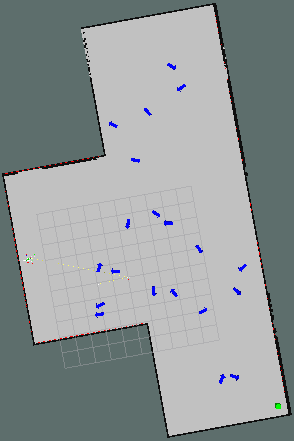
\includegraphics[width=0.7\textwidth]{figures/people.png}
    \caption{Example setting }
    \label{fig:exp_setting}
  \end{subfigure}
  \hspace{10mm}
  \begin{subfigure}[b]{0.435\columnwidth}
  \hspace{4mm}
    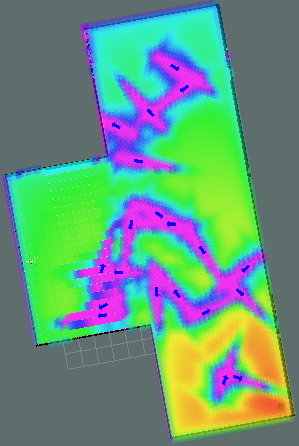
\includegraphics[width=0.7\textwidth]{figures/cost_f.png}
    \caption{Cost function}
    \label{fig:cost_f}
  \end{subfigure} 

  %\vspace{-3mm}
  \caption[An instance of the randomised social navigation task, and its cost function.]{(a) An instance of the randomised social navigation task. Arrows denote the position and orientation of people in the scene. The robot is on the lefthand side of the map and the green box in the bottom right denotes the goal location. (b) The corresponding cost function for the random scenario. Red denotes \emph{low} cost, while purple denotes \emph{high} cost.}

  %\vspace{-3mm}
  \label{fig:setting}
  \end{figure}


	\subsubsection{Evaluation}

	To evaluate the effectiveness of our algorithms we employ both quantitative as well as qualitative comparisons.

	To quantitatively assess the quality of our algorithms, we generate a dataset $D$ by planning near-optimal paths from an initial configuration $s_o$ to a goal configuration $s_g$ under a ground-truth cost function $c_{gt}()$ derived from respective ground-truth weights $\mathbf{w}_{gt}$. A fully optimal path can only be derived only asymptotically in terms of either time  for RRT$^*$, or resolution for A$^*$. In practice, however, we found that planning for 60 seconds using  RRT$^*$  achieves a path that is nearly optimal, as running longer leads to negligible changes in path cost. 

	The resulting ground truth dataset is extremely useful for evaluation. For each path $\zeta$ generated by the learner, we know its cost under the ground-truth cost function is simply  $\mathbf{w}_{gt}\mathbf{F}(\zeta)$. Furthermore, we can compute the cost difference between the generated path and the example path:
	\begin{equation}
		Q(\zeta,\zeta_i,\mathbf{w}) = \mathbf{w}(\mathbf{F}(\zeta)-\mathbf{F}(\zeta_i)), \label{eq:obj_eval}
	\end{equation}
which is our primary performance metric.  Note that, if the demonstration path $\zeta_i$ is optimal under $\mathbf{w}$, then $Q(\zeta,\zeta_i,\mathbf{w})>=0$.

For our experiments, the ground-truth weights $\mathbf{w}_{gt}$ were chosen to induce a cost function that penalises passing in front of people. In addition, small weights were added to the other two Gaussian functions for each each individual person, as well as both linear and exponential penalisation of the distance from the goal, so that the resulting cost function, shown in Figure \ref{fig:cost_f}, would not be too trivial. 

We also measure the time per iteration of each learning algorithm.  All algorithms were implemented in Python, share similar functions, and were not optimised for speed apart from the caching scheme in RLT$^*$.

	We also perform qualitative evaluation of the algorithms by visually comparing the learned cost functions for each algorithm and the paths they generate against the ground truth cost function and the demonstration paths.

	\subsubsection{Results}

	Our dataset $D$ consists of 20 trajectories at random social situations within the social environment shown in Figure \ref{fig:exp_setting}, using the cost function shown in Figure \ref{fig:cost_f}. Half of these trajectories make up the training dataset $D_{train}$ and the other half the test dataset $D_{test}$. After being trained on $D_{train}$, the performance of a cost function is evaluated on $D_{test}$ using \eqref{eq:obj_eval}. The process is repeated four times for the same dataset but with different random compositions of $D_{train}$ and $D_{test}$. We report both the mean and standard error across the different trajectories in the test and training sets, for each iteration in Figures \ref{fig:train_results} and \ref{fig:test_results}. 

We report results for RLT$^*$, RLT$^*$ without caching, and MMP with A$^*$ at grid resolutions of 0.8 and 0.3 metres.  For RLT$^*$, we set the number of sampled points $p=2500$. For RLT$^*$ without 
caching, we cap planning at 12$s$, which is about how long RRT$^*$ plans for when $p=2500$.  Note 
that this is much less planning time than the 60$s$ used to generate the demonstrations.
 All learning algorithms were initialised using a cost function that only favours shortest paths.

The results show that both versions of RLT$^*$ always outperform both versions of MMP with A$^*$. This can be attributed to the fact that the underlying RRT$^*$ planner is not confined to work on a fixed grid, allowing it to generate paths that are closer to optimal. This is further reinforced by the increased performance as the grid resolution decreases allowing MMP$_{0.3}$ to approach the performance of RLT$^*$. Standard error rates are similar across methods.

	Table \ref{tab:time} shows the average planning time per learning iteration and the total learning time for all algorithms, along with their average cost difference on the test set at convergence. Comparing RLT$^*$ with and without caching shows that the cached version is much faster without a significant cost in performance. Furthermore both algorithms, although slower than MMP$_{0.8}$, are faster than MMP$_{0.3}$. This means that, even if a higher resolution MMP  was able to match the performance of RLT$^*$, it would be much slower. Furthermore, there is large variance in planning time for MMP$_{0.3}$. At the start of learning, the initial cost function is very simple and and only involves the distance from the goal location. Under this cost function, planning is quick, because a simple heuristic that simply takes into account the distance from the goal is a  good approximation to the cost-to-go. As learning proceeds, however, the cost function becomes more complex, and this simple heuristic, although admissible, is no longer tight. This requires the A$^*$ planner to expand many more states before an optimal path is found. We can see therefore that MMP with A$^*$ scales poorly, not only the size of $S$, but also in the complexity of the cost function. By contrast, the probabilistic nature of RLT$^*$ makes it less susceptible to these pathologies.  

	For a qualitative comparison, we look to Figures \ref{fig:path_compare} and \ref{fig:cfs}. Figure \ref{fig:path_compare} shows a demonstrated path (black) along with the paths generated by three of the four algorithms. Note the effect of planning on a coarse grid in the case of MMP$_{0.8}$ (green). We can also see that RLT$^*$ (red) more faithfully replicates the example path. Figure \ref{fig:cfs} compares the ground truth cost function (Figure \ref{fig:get_cf}) against the learned cost functions for  MMP$_{0.3}$ and RLT$^*$ (Figures \ref{fig:astar03_cf}, \ref{fig:rrt_cf}). This comparison shows that  MMP$_{0.3}$ overestimates the cost related with the distance from the goal, i.e., the cost increases faster as we move away from the goal. This yields paths that reach the goal earlier, possibly accounting for the small difference in performance between the two algorithms. 

\begin{figure}[tbh]
	\centering
%	\hspace{-5cm}
      \begin{subfigure}[b]{0.45\columnwidth}

    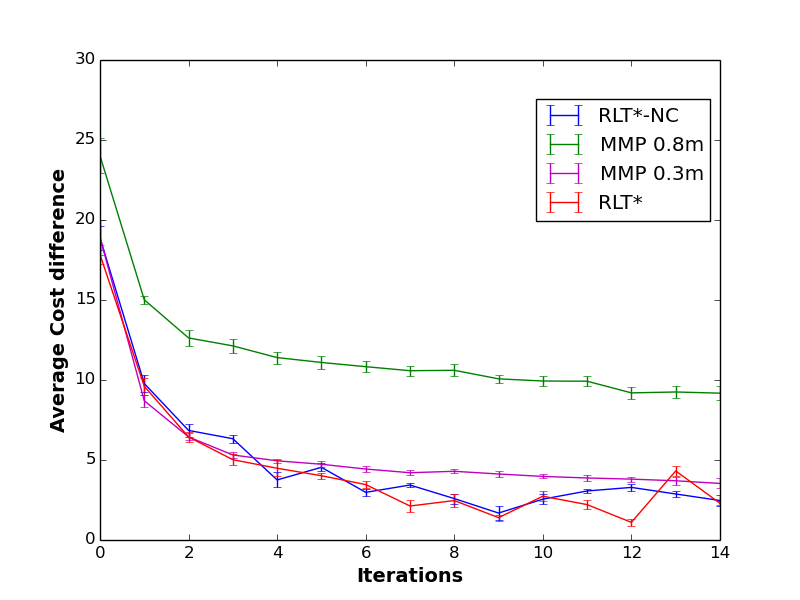
\includegraphics[clip=true,width=1.\textwidth]{figures/cost_diff_train.png}
    \caption{Train}
    \label{fig:train_results}
  \end{subfigure}
 % \hspace{5mm}
  \begin{subfigure}[b]{0.45\columnwidth}
    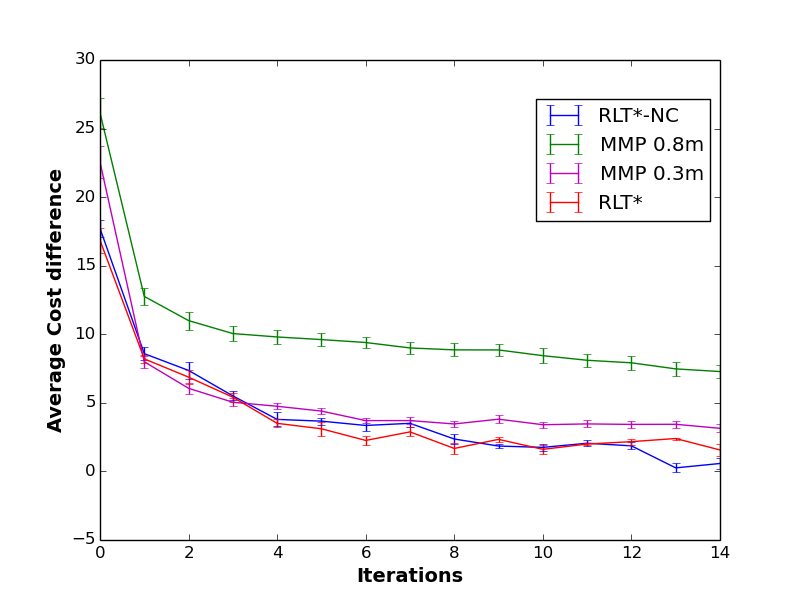
\includegraphics[clip=true,width=1.\textwidth]{figures/cost_diff_val.png}
    \caption{Test}
    \label{fig:test_results}
  \end{subfigure} 

  %\vspace{-3mm}
  \caption[Train and test set average cost difference, for 15 iterations.]{Train and test set average cost difference, for 15 iterations. Error bars represent standard error over four independent runs on shuffled versions of the data. (RLT$^*$-NC is RLT$^*$ without caching.)}
  %\vspace{-3mm}
  \label{fig:results}
\end{figure}



	\begin{table}[]
  \centering
	\scalebox{1.}{
	\begin{tabular}{|l|l|l|l|l|}
	\hline
	               & MMP$_{0.8}$     & MMP$_{0.3}$       & RLT$^*$-NC  & RLT$^*$ \\ \hline
	Iteration (s) & 1.83(0.79) & 20.93(12.14) & 12(0) & 5.87(0.50)  \\ \hline
	Learning (s) & 275.2      & 3140.6       & 1808  & 911.7       \\ \hline
	$Q(\zeta,\zeta_i,\mathbf{w}_{gt})$ & 7.28      & 3.14       & 0.57  & 1.57       \\ \hline
	\end{tabular}}
	\caption[Per iteration and total learning times.]{Per iteration and total learning times for our proposed algorithms and the baselines (RLT$^*$-NC is RLT$^*$ without caching.). Values in parentheses denote standard deviation.}
	\label{tab:time}
	\end{table}


	\begin{figure}
	\centering
	%\vspace{-3.3mm}
	    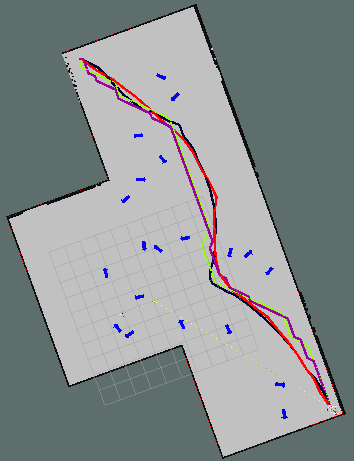
\includegraphics[width=0.3\textwidth]{figures/path_compare.png}
	%\vspace{-4mm}
	  \caption[Qualitative comparison of paths.]{Qualitative comparison of paths. Goal is at the top left, robot begins on the bottom right. Black: demonstration path. Red: RLT$^*$. Green: MMP$_{0.8}$, Magenta: MMP$_{0.3}$ }
	  \label{fig:path_compare}
	\end{figure}


	\begin{figure}[tbh]
	\hspace{5mm}
      \begin{subfigure}[b]{0.309\columnwidth}
    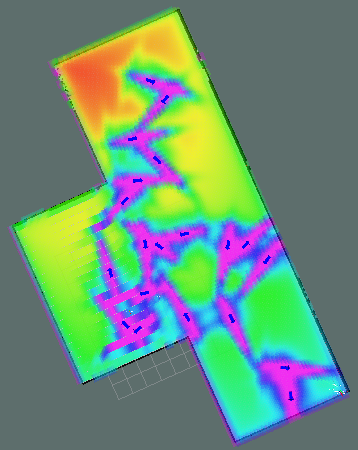
\includegraphics[width=1.\textwidth]{figures/gt_ct.png}
    \caption{Ground truth}
    \label{fig:get_cf}
  \end{subfigure}
  %\hspace{1mm}
  \begin{subfigure}[b]{0.30\columnwidth}
    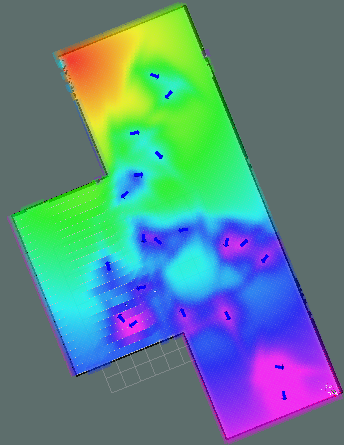
\includegraphics[width=1.\textwidth]{figures/astar03.png}
    \caption{MMP$_{0.3}$}
    \label{fig:astar03_cf}
   \end{subfigure}
   %\hspace{1mm}
  \begin{subfigure}[b]{0.305\columnwidth}
    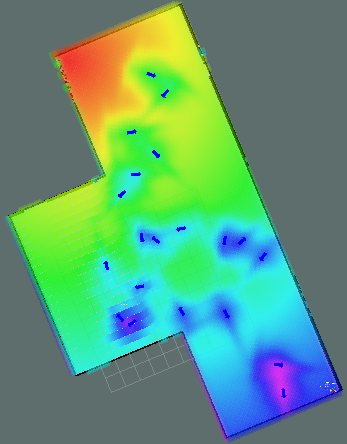
\includegraphics[width=1.\textwidth]{figures/rrt_cf.png}
    \caption{RLT$^*$}
    \label{fig:rrt_cf}
  \end{subfigure} 
  	  \caption{Ground truth and learned cost functions using MMP$_{0.3}$ and RLT$^*$.  \label{fig:cfs}}
  \end{figure}


\subsection{Conclusion and Future Work}
In this section, we proposed Rapidly Exploring Learning Trees (RLT$^*$), which learns the cost functions of Rapidly Exploring Random Trees (RRT) from demonstration, thereby making inverse learning methods applicable to more complex tasks. Our approach extends the Maximum Margin Planning to work with RRT$^*$ cost functions. Furthermore, we proposed a caching scheme that greatly reduces the computational cost of this approach. Experimental results on real and simulated data from a social navigation scenario showed that RLT$^*$ achieves better performance at lower computational cost than existing methods.

 Although our experimental comparison used A$^*$ as a baseline, RLT$^*$ is also well suited to situations where deterministic planners naturally fail, e.g., a manipulator with many degrees of freedom. A clear avenue for future work is to design learning algorithms that explicitly take into account the probabilistic nature of RRT$^*$. We also plan to evaluate RLT$^*$ on data using the actual TERESA robot. This will in turn allow us to deploy the learned cost function on the robot. Finally we will combine learning from failure, introduced in Section \ref{sec:irlf} with the RLT$^*$ and evaluate its performance on the TERESA robot.

\clearpage

\section{Cost Functions for Social Conversation}
\label{sec:cost_functions}

The task of engaging in social conversation through the TERESA robot has different control objectives and is subject to different social constraints than the task of social navigation. Therefore, the cost functions that will be used within the autonomous social conversation behaviours of the robot must be learned separately from those of social navigation.

As discussed in Deliverable 5.1 \cite{d5.1}, there are multiple sources of feedback from which some measure of the social adequacy of the behaviours of the robot may potentially be inferred. Namely:
\begin{itemize}
\item The reactions of the telepresent visitor\footnote{We here use the same terminology for the conversation task as in previous deliverables. Namely, the ``visitor'' is the person using the robot remotely; and the ``interaction targets'' are any persons which are physically co-present with the robot and engaged in the conversation.};
\item The reactions of the interaction targets engaged in conversation with the visitor through the robot;
\item The demonstrations of social (and possibly asocial) behaviour by human experts. 
\end{itemize}

In this section, we describe our progress of learning social cost functions for social conversation through feedback that is provided from 1) the visitor and 2) the interaction targets. Learning social cost functions for social conversation from expert demonstrations falls under the scope of the IRL methods described in Section \ref{sec:irlf}, which can also be applied in this context, and constitutes future work.

Our main contributions in this topic can be summarized as follows:
\begin{itemize}
\item In Section \ref{sec:initial_experiment}, we describe local experiments that were performed at the University of Amsterdam for a conversation scenario with the TERESA robot in various conditions, where we recorded explicit negative feedback from the visitor. This data was used to extract a measure of social cost related to proxemics form the perspective of the visitor. This cost function based on explicit feedback complements the cost functions that we had described in \cite{d5.1} that were based on implicit feedback from the visitor;
\item In Section \ref{sec:group conversations}, we present an analysis of the data that was collected by the TERESA consortium partners at the University of Twente (UT), through the experimental process described in Deliverable 3.1 \cite{d3.1}. We processed these data and extracted from them a measure of social cost related to proxemics from the explicit qualitative feedback provided by the participants of that study.
\end{itemize}

\subsection{Local Experiment on Social Conversation}
\label{sec:initial_experiment}

An experiment regarding social conversation with the TERESA robot was conducted at the University of Amsterdam, between <fill in dates>\todo{confirm the dates w/ Richard}. The purpose of this experiment was twofold: firstly, to record both implicit and explicit feedback of the visitor and an interaction target to the behaviour of the robot under controlled conditions, so as to enable the learning of cost functions that are representative of the social acceptability of those behaviours; secondly, to determine an appropriate representation of the state space for a decision-theoretic representation of the control task during autonomous social conversation.

\subsubsection{Experimental Setup and Procedure}

The general set-up of the local social conversation experiment followed closely that of the social navigation experiments that were performed previously in the project. In particular, a ``Wizard of Oz'' setup was also used, where the robot is controlled by an \textit{expert} located in an isolated area. This expert acted with different degrees of quality in order to trigger a response to the behaviour of the robot. The layout of the experiment (two rooms with an additional separated area for the expert) can be seen in Figure \ref{fig:experiment_setup}.

\begin{figure}
    \centering
    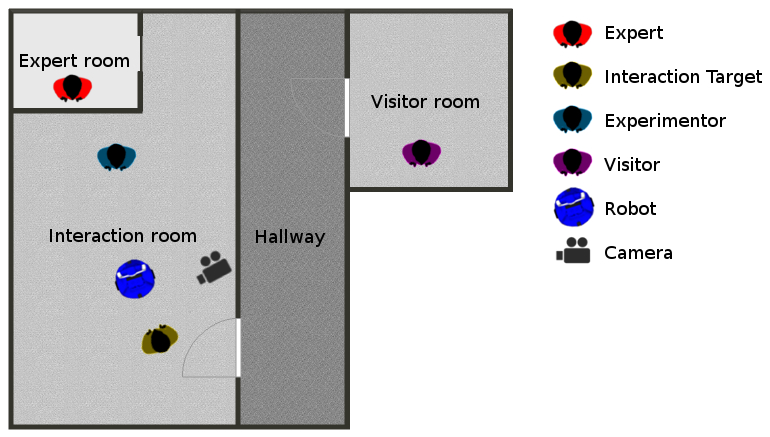
\includegraphics[width=0.8\textwidth]{figures/experiment_setup_new.jpg}
    \caption{Layout of the initial experiment}
    	\label{fig:experiment_setup}
\end{figure} 

In terms of hardware, the experimental setup was distributed across five networked locations:
\begin{itemize}
\item The TERESA robot;
\item The computer running the Giraff Interface, used by the visitor to communicate with the interaction target through the robot;
\item The computer used by the expert to control the robot;
\item An auxiliary computer to record the data captured by a Dalsa GENIE camera that was directed towards the face of the visitor, in accordance with the general TERESA system architecture;
\item An auxiliary computer relaying a feed from an overhead camera installed in the interaction room. The camera was used to give the expert a better overview of the room, and used for later validation of the data.
\end{itemize}

The visitor was asked to give explicit feedback, in the form of keyboard presses, whenever the robot performed behaviours which were socially unacceptable.

Each experimental run involved two subjects, and was split into three phases. In the first of these phases, we intended to study the reactions of the participants to approach/retreat behaviours by the robot, similarly to what had been performed in the inductive user study described in Deliverable 3.1 \cite{d3.1}, as well as to study the correlation between the range of operation of the robot (its distance to the interaction target) during conversation, and social acceptability. To achieve this, at regular intervals during the experiment, we alternatingly performed the following behaviours in random order:
\begin{itemize}
\item The robot moved closer or farther away from the interaction target, at the discretion of the expert. The expert was instructed to attempt to elicit reactions from the participants, and therefore explored a varied range of distances to the interaction target during conversation, both within as well as outside of the expected operational conditions for the TERESA robot. For instance, at times the expert moved the robot as close as possible to the interaction target without placing the subject in danger of collision; and also placed the robot as far as physically possible from the interaction target;
\item The interaction target was asked to move to a distance with respect to the robot which he/she felt was:
  \begin{itemize}
  \item Normal for a one-to-one conversation;
  \item As close as possible without becoming socially unacceptable;
  \item As far as possible without becoming socially unacceptable.
  \end{itemize}
\end{itemize}

The visitor and the interaction target were instructed to maintain a normal conversation throughout each experimental run, and were informed \emph{a priori} that, at the request of the experimenter, either the robot or the interaction target would need to move (but not both simultaneously).

In the second phase of each experimental run, the visitor and interaction target continued the conversation while the expert executed various behaviours at different levels of perceived social acceptability. Acceptable behaviours include maintaining the correct body pose and correctly changing the distance based on social cues (e.g. hearing problems); whereas unacceptable behaviours include suddenly turning away from or randomly changing the distance to the interaction target. In this phase we focused especially on eliciting explicit negative feedback from the visitor by changing the orientation of the robot during conversation.

The third and final phase of the experimental runs explored the influence of communication difficulties on proxemics. Communication problems can be prevalent in the elderly due to hearing problems. To simulate such a situation, we introduced artificial background noise (i.e. sounds of a cafeteria) at various levels during the experiment, and repeated the approach/retreat conditions of the first phase. After these were performed, the interaction target was asked to sit down, while the expert was still free to change the distance of the robot. The rationale for this step was that, while sitting down, people may exhibit characteristic reactions to hearing difficulties which we intended to record (such as leaning forward, as it had been identified by UT in their own experiments).

The visitor and interaction target were then asked to switch places. Therefore, we performed two experimental runs for each pair of subjects. At the end of the two experimental runs, an interview was conducted with the subjects to obtain some additional insight on the behaviour of the robot.

In total, $12$ subjects were involved in our local experiments, which consisted of a mix of student and faculty voluteers.

\todo[inline]{Joao: I'd like to have a link to a video of the experiments.}

\subsubsection{Results}
\label{sec:social_results}

{\bf A Common Representation of the State Space for Autonomous Social Conversation}
\label{sec:defining_the_state-space}

In the previous deliverable in this Work Package (Deliverable 5.2 \cite{d5.2}), we have discussed in detail the relevant control variables for the TERESA social conversation task, and proposed a set of high-level actions for this task. Notably, we have concluded that most of the actions involved in social conversation require controlling the relative distance and bearing between the robot and one or more interaction targets, through the linear and angular velocity of the base of the robot. This conclusion was supported by the inductive user study conducted by UT in Deliverable 3.1 \cite{d3.1}, which demonstrated that the distance and bearing of the robot with respect to the interaction targets are both variables of interest in order to maintain social acceptability. 

Naturally, the most useful representations of social cost functions in this conversation task should be defined over the same variables which are to be controlled by the autonomous behaviours of the robot. Therefore, our aim is to obtain a representation of social cost as a function of distance and bearing w.r.t the interaction target(s), and potentially also the linear and angular velocity of the robot. These are inherently continuous physical variables. Specifically, given the position of the interaction target as $p_I = [x_I\,\,y_I]^T$ and of the robot $p_R = [x_R\,\,y_R]^T$ in some common fixed frame, we define \emph{distance} in the conversation task as $\rho = ||p_I - p_R||$ where $||\cdot||$ is the Euclidean norm, and \emph{bearing} as $\phi = \arctan \frac{y_I - y_R}{x_I - x_R} - \theta$, where $\theta\in(-\pi,\pi]$ is the orientation of the robot in the same fixed frame. We also take the linear and angular velocity of the robot to be $v = dp_R/dt$ and $w = d\theta/dt$ respectively.

However, we note that the control solutions that we intend to develop for the autonomous behaviours of the robot during social conversation are based on decision-theoretic concepts, and it is not straightforward to use continuous representations of states and actions in these frameworks, since that would make these approaches intractable. Therefore, it is useful to first identify a compact, discretized representation of the state and action spaces, and to represent our cost functions in the same domains.

The study of proxemics \cite{hall1966hidden} has identified a discrete set of distance intervals for different types of interaction between humans. These distances are defined as the \emph{personal}, \emph{social}, and \emph{public} proxemic zones. This lends support to the hypothesis that a similar discrete representation of the distance space would be a natural basis for the domain of this variable within the TERESA social conversation task. In doing so, however, it is important to test the hypothesis that the available results on proxemics are also applicable to the TERESA social conversation task -- that is, that the fact that the users are interacting through a robot does not noticeably influence their proxemic zones. Therefore, based on our experimental data, we first attempted to learn a discretized proxemics-based representation of the distance space.

During our experimental runs, we collected the distances between the robot and the interaction target, as measured by the robot's laser range-finder. For the purpose of state space identification, the relevant portion of this dataset concerns the segments of the experimental runs where we asked the subjects to approach the robot to what they considered to be the normal, minimum and maximum interaction distances. In particular, we extracted the set of final distances of the subjects after their approaches to the robot, as $R = \{\rho_1, \rho_2,\ldots,\rho_N\}$, in the scenarios where there were no hearing difficulties. We then ran $K-$means clustering \cite{hartigan1979algorithm} with $K=3$ on dataset $R$ to identify the centroids of these interaction distances. The centroids of the resulting clusters, based on 31 approaches, are as follows:
\begin{align*}
\rho_{close} = 0.71m,\quad \rho_{normal} = 1.16m,\quad \rho_{far} = 1.68m.
\end{align*}

Furthermore, let $\rho_{hprob}$ represent the average distance at which interaction targets approach the robot \emph{normally} under the presence of background noise, so that the robot was within their perceived social space. According to our data, we have that $\rho_{hprob}=0.93m$. In this case there was no significant difference in our data regarding the values for the personal and public proxemic zones.

We then define the discrete \emph{distance state} of the robot during social conversation as $d\in\{d_{personal},d_{social},d_{public}\}$.
 Let $F_{\rho}:\{d_{personal},d_{social},d_{public}\}\rightarrow\{\rho_{close}, \rho_{normal}, \rho_{far}\}$ be a bijection where $F_\rho(d_{personal}) = \rho_{close}$,  $F_\rho(d_{social}) = \rho_{normal}$ and  $F_\rho(d_{public}) = \rho_{far}$. Then, during execution, and in the absence of background noise, the distance state of the robot can be determined as:
 \begin{align*}
   \argmin\limits_{d\in\{d_{personal},d_{social},d_{public}\}} |\rho_t-F_\rho(d)|,
 \end{align*}
where $\rho_t$ is the real-valued distance at time $t$.

In the presence of background noise, a similar mapping $F^{hprob}_{\rho}:\{d_{personal},d_{social},d_{public}\}\rightarrow\{\rho_{close}, \rho_{hprob}, \rho_{far}\}$ can be used. By selecting the appropriate interaction distance values depending on whether or not there is perceived background noise, the robot can move closer to the interaction targets if it is within their social proxemic range.

The bearing between the robot and the interaction target should also be discretized. However, contrarily to the distance, there are no known results in the study of proxemics that can inform our discretization. A straightforward solution would be to divide the full angular range into equally-sized intervals. This would however lead (depending on the size of these intervals) to either many states with high precision or a small amount of states with low precision. A better solution is to take into consideration the physical shape of the robot and the capabilities of its sensors. This suggest that the angular discretization in front of the robot should have a higher resolution, since 1) the sensors of the robot have a limited field-of-view and are more accurate within that region and 2) the viewability of the screen of the robot is also limited. The social cost of standing beside or behind the robot should therefore not differ much, since the screen can not be viewed from those angles, making teleconferencing impossible.

Based on this idea, we have divided the angular range in front of the robot into steps of 10 angular degrees in width up to $50º$. That is, let
\begin{align*}
  \Phi:=\{-50º,-40º,-30º,-20º,-10º,0º,10º,20º,30º,40º,50º\},
\end{align*}
and $F_\phi:\{b_i\}_{i=1,\ldots,11}\rightarrow \Phi$ where $\{b_i\}_{i=1,\ldots,11}=:B$ is the discrete \emph{bearing state} space. Then the bearing state at time $t$ is defined as:
\begin{align*}
  b(t) = \argmin_{b\in B}|F_\phi(b) - deg(\phi_t)|,
\end{align*}
where $\phi_t$ is the bearing at time $t$, and $deg(\phi_t)=\phi_t\times\frac{180}{\pi}$.

Another important fact regarding the bearing is that the robot is symmetric and the conversation task, \emph{a priori}, has no reason to favor one angular direction over the other. Therefore we assume that the social cost should also be symmetric with respect to the bearing (i.e. the cost at the left of the robot should equal the cost at the right of the robot). This hypothesis is also proven in Section \ref{sec:group_result} and leads to requiring less experimental data and removes possible biases during the experiments. During execution, however, the actions of the robot naturally should depend on the actual direction of the interaction target. In Figure \ref{fig:state_viz}, the different angular states are reperesented in grayscale, and this symmetry can also be seen.


\begin{figure}
    \centering
    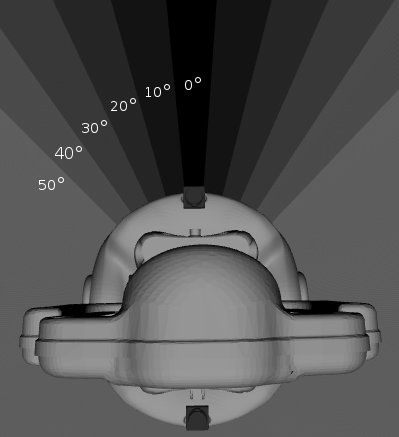
\includegraphics[width=0.4\textwidth]{figures/state_viz.png}
    \caption[Representation of the bearing state.]{Representation of the bearing state. Darker shades of grey correspond to lower bearings. In this representation, the bearing states to the right and left of the robot are aliased. This is the representation that is used as a basis for the social cost w.r.t. the bearing. However, during execution, the robot should discriminate between these different directions.}
    	\label{fig:state_viz}
\end{figure}

{\bf Social Cost from Explicit Negative Feedback}

During our local experiments, we collected a total of 65 instances of explicit negative feedback from the participants in the role of visitor, in the form of key presses. As each test subject provided a different total amount of explicit feedback (some participants were more reserved than others in their use of the feedback functionality), a normalization was applied to the amount of feedback provided by each user. In Figure \ref{fig:button_presses}, the normalized relative frequency of explicit feedback by the visitors is plotted against the states of the robot, as per the state space description described in the previous section. This representation makes it evident that there is a very sparse distribution of key presses over states. Since there is insufficient data to fairly estimate the frequency of negative feedback at each particular distance-bearing pair, this representation makes it seem (incorrectly) that higher bearing values would be associated with lower social cost, which is not only unintuitive, but also contradicts UT's original findings.

However, when looking purely at the distribution of explicit feedback over distances (marginalizing out the influence of bearing), a clear distribution that our intuition also supports can be observed, which is represented in Figure \ref{fig:distance_cost}. Here we can see that, based on the explicit feedback, being at the distance which most users considered to be ``normal'' yield the lowest likelihood of receiving negative feedback.

\begin{figure}
    \centering
    \begin{subfigure}[b]{0.45\textwidth}
        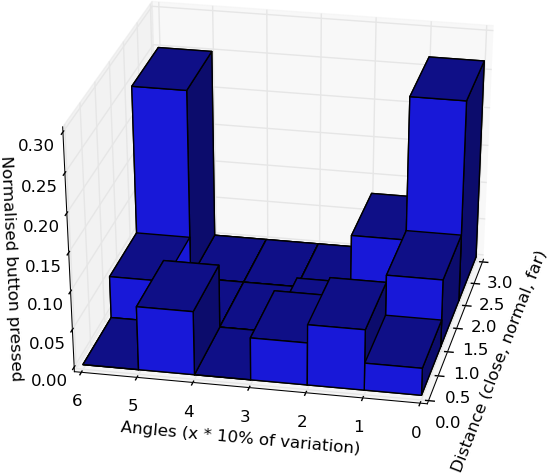
\includegraphics[width=\textwidth]{figures/key_presses_normalised_cropped.png}
        \caption{Explicit feedback from pilot}
        \label{fig:button_presses}
    \end{subfigure}
    \begin{subfigure}[b]{0.45\textwidth}
        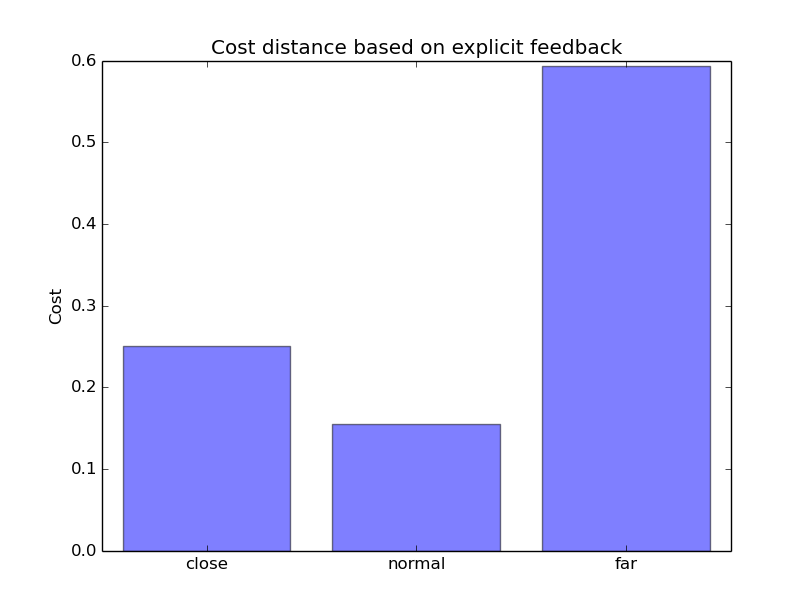
\includegraphics[width=\textwidth]{figures/Distance_cost.png}
        \caption{Cost function based on distance}
        \label{fig:distance_cost}
    \end{subfigure}
    \caption{Explicit feedback from pilot}
    \label{fig:button_presses_cost}
\end{figure}

Given the distance intervals that were estimated previously from the approach data, the social cost based on the distance can be extracted and visualized as shown in Figure \ref{fig:state_res_distance_1}. Here, the interaction target is indicated by the purple human like shape, where the arrow indicates its orientation. The different distance states $\{d_{personal}, d_{social}, d_{public}\}$ are indicated by the circles surrounding the interaction target. Note that the actual distance values corresponding to each of these states depend on the presence or absence of hearing problems.

\begin{figure}
    \centering
    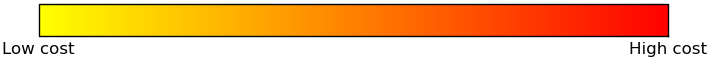
\includegraphics[width=0.6\textwidth]{figures/colour_bar.png}
    \begin{subfigure}[b]{0.45\textwidth}
        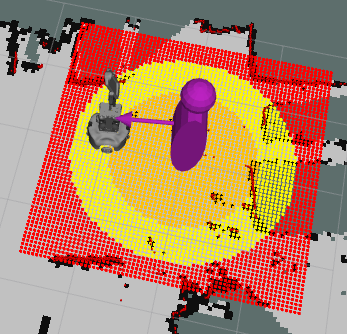
\includegraphics[width=0.8\textwidth]{figures/cost_function_no_hearing_problems.png}
        \caption{Normal situation}
        \label{fig:state_res_distance_1}
    \end{subfigure}
    \begin{subfigure}[b]{0.45\textwidth}
        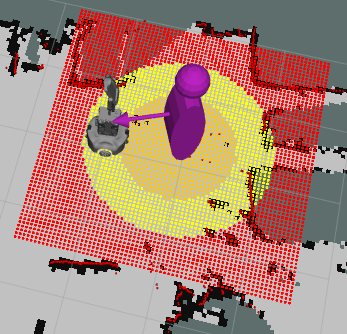
\includegraphics[width=0.8\textwidth]{figures/cost_function_hearing_problems.png}
        \caption{With hearing problems\\ / low communication quality}
        \label{fig:state_res_distance_2}
    \end{subfigure}
    \caption{State representation (distance)}
    \label{fig:state_res_distance}
\end{figure}

In Figure \ref{fig:cost_function_1}, we show an approach to the interaction target that was performed while the robot was being controlled by the expert. The distance at which the expert finishes the approach can be seen in Figure \ref{fig:cost_function_2}, and lies within the normal distance state where our defined cost function also gives the lowest cost.

\begin{figure}
    \centering
    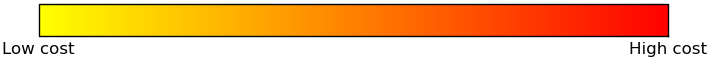
\includegraphics[width=0.6\textwidth]{figures/colour_bar.png}
    \begin{subfigure}[b]{0.45\textwidth}
        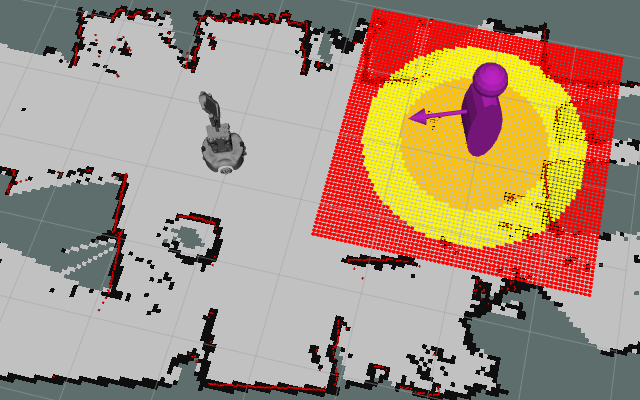
\includegraphics[width=\textwidth]{figures/cost_function_1.png}
        \caption{Initial position}
        \label{fig:cost_function_1}
    \end{subfigure}
    \begin{subfigure}[b]{0.45\textwidth}
        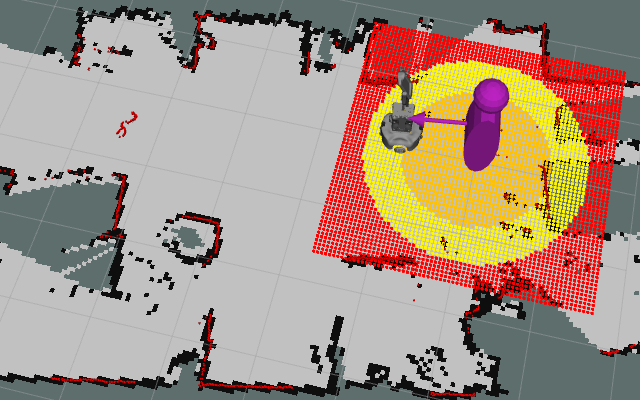
\includegraphics[width=\textwidth]{figures/cost_function_2.png}
        \caption{Final position after the approach}
        \label{fig:cost_function_2}
    \end{subfigure}   
    \caption[One of the recorded approaches to the interaction target.]{One of the recorded approaches to the interaction target while the robot was controlled by an expert. The identified distance space partitions are overlayed on the interaction target. The expert tended to position the robot in the zone identified as the ``social'' proxemic space of the interaction target (yellow).}
    \label{fig:cost_function}
\end{figure}

%{\bf Social Cost from Implicit Feedback}
%If there is time

\subsection{Group conversations}
\label{sec:group conversations}

The consortium partners at UT have also conducted an experiment which focused on social positioning of the TERESA robot within group conversations. During this experiment, which is described in Deliverable 3.1 \cite{d3.1}, our partners focused on studying the proxemics in the social conversation task through the theory of F-formations \cite{kendon1990conducting} (i.e. different spatial arrangements for persons during group conversations) for situations with multiple interaction targets. Our partners have granted us access to their datasets, consisting of robot trajectories and user scores collected during group conversation episodes. We have used this dataset to learn social cost functions for social conversation from the feedback given by the interaction targets.

\subsubsection{Results}
\label{sec:group_result}

The full description of the experimental setup and protocol of the experiments performed by UT can be found in \cite{d3.1}. In summary, each experimental run consisted of three phases: an approach phase, during which the pilot drove the robot to a group of interaction targets; a conversation phase, during which the pilot maintained an interaction with the group; and a retreat phase. At the end of the experimental run, the users scored the quality of the interaction on a $1-7$ numerical scale where $7$ represents an interaction that is completely socially acceptable, and $1$ a socially unacceptable interaction.

As in the case with a single interaction target, we are also interested in obtaining an appropriate state space representation for group conversation scenarios. The theory of F-formations suggests that, in group conversations involving three or more persons, the participants tend to position themselves facing the geometric center of the convex hull of their formation \cite{kendon1990conducting}. This formation, for the social conversation task, is exemplified in Figure \ref{fig:F-formation_experiment}. This prior knowledge tells us that the distance and bearing of the robot with respect to the center of a group should be included in the target variables to control during a group conversation task. The results of UT have shown that deviations in bearing, in particular, are significantly correlated with the score given by the users at the end of the interaction. However, these two variables may not be sufficient -- we must also consider the possible influence of the distance and bearing with respect to each participant as a potential source of social cost.

\begin{figure}
    \centering
    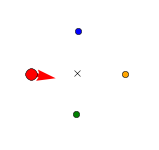
\includegraphics[width=0.4\textwidth]{figures/o-space_twente_data.png}
    \caption[An example of the F-formation during group conversation experiments.]{An example of the F-formation during group conversation experiments (robot in red, participants in blue, green and yellow and the center of the group is denoted by a cross).}
    	\label{fig:F-formation_experiment}
\end{figure} 

In order to determine whether or not we should include the distance and bearing with respect to each individual participant in our representation of the state space for the conversation task, we performed a statistical analysis of the influence of these variables on the resulting grade provided by each participant after the interaction task.

More concretely, we first organized the data by grouping the scores provided by the participants into $6$ different classes, corresponding to $6$ possible bearing states $b_0,\ldots,b_5$. Each state $b_i$ corresponds to an absolute deviation in bearing with respect to the center of the group of $i\times 10$ degrees (with state $b_5$ including all possible deviations greater than $50º$). The scores were split into each class according to the average bearing of the robot with respect to each subject during the conversation phase. This was possible since the pilot rarely moved the robot during the conversation phase, maintaining its bearing at a relatively constant value. Our proccessed dataset then consists of sets of samples $U_i = \{u_{i,1},u_{i,2},\ldots,u_{i,N_i}\}$ with $i\in\{0,\ldots,5\}$, where each $u_{i,j}\in U_i$ represents a score in the range $\{1,\ldots,7\}$ given by one of the participants, given that the bearing state with respect to that participant was $b_i$.

We then tested the following null hypothesis:
\begin{align*}
 H_0 := & \text{ \textit{The bearing state with respect to the individual participants}}\\
        & \text{ \textit{does not influence the distribution of scores.}}
\end{align*}

Due to the different sample sizes of each set $U_i$, and the non-normality of the distribution of scores in each class, we opted to use the Kruskal-Wallis for statistical significance. The result of this test based on hypothesis $H_0$ was $p = 0.14$, which suggests that there is not a statistically significant difference between the sample sets at least at a level of significance of $10\%$. This leads us to conclude that we do not need to represent the bearing state with respect to each individual participant in a group conversation scenario as part of our state variables for the respective control task. Our dataset and the resulting expected values for each class are represented in Figure \ref{fig:cumulative1}. This visual representation also makes it clear that the distribution of scores is relatively constant as a function of the individual bearing state.

We furthermore attempted to demonstrate that the bearing state with respect to the group as a whole is indeed a relevant variable, and that the proposed discretization captures the influence of this variable on the scores provided by the participants. To achieve this, we re-organized the data so that each $u_{i,j}\in U_i$ now represents the score of a participant given that the bearing state \emph{with respect to the center of the group} was $b_i$. This allows us to test the hypothesis:
\begin{align*}
 H_1 := & \text{ \textit{The bearing state with respect to the the center of the group}}\\
        & \text{ \textit{does not influence the distribution of scores.}}
\end{align*}

The Kruskal-Wallis test based on this hypothesis results in $p = 1.36\mathrm{e}{-4}$, which means that this hypothesis is rejected even at a confidence level of $1\%$, and that the bearing relative to the center of the group, on our proposed discretization, does indeed make a difference in the grade given by the participants. The probability distribution over scores for each class in this case is represented in Figure \ref{fig:cumulative2}.
%(25.058705342300826, 0.00013574376253141289)

%%%%%%%%%%%%%%%%%%%%%%%%%%%%%%%%%%%%%%%%%%%
%
% Worked out till this point
%
%%%%%%%%%%%%%%%%%%%%%%%%%%%%%%%%%%%%%%%%%%
 \begin{figure}
    \centering
    \begin{subfigure}[b]{0.45\textwidth}
        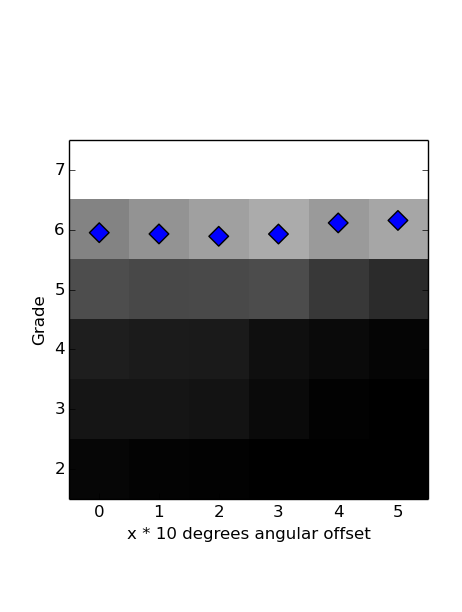
\includegraphics[width=\textwidth]{figures/grade_cumulative.png}
        \caption{Individual bearing state}
        \label{fig:cumulative1}
    \end{subfigure}
    \begin{subfigure}[b]{0.45\textwidth}
        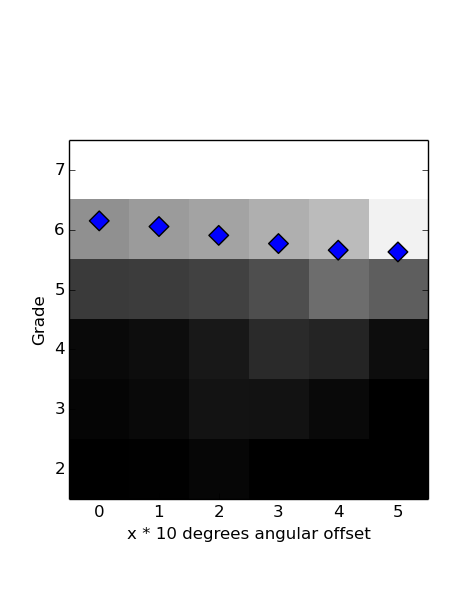
\includegraphics[width=\textwidth]{figures/grade_cumulative_COM.png}
        \caption{Group bearing state}
        \label{fig:cumulative2}
    \end{subfigure}
    \caption[Cumulated probabilities over grades as a function of the bearing state.]{Cumulated probabilities over grades as a function of the bearing state (\subref{fig:cumulative1}) of each individual participant and (\subref{fig:cumulative2}) with respect to the geometric center of the group. The probabilities are represented in grayscale, where a value of $1$ corresponds to white (the cumulative probability of score $7$ is always $1$), and a value of $0$ corresponds to black. The expected value of the grade for each class is denoted by a blue diamond.}
    \label{fig:cumulative_probs}
\end{figure}

 \begin{figure}
    \centering
    \begin{subfigure}[b]{0.45\textwidth}
        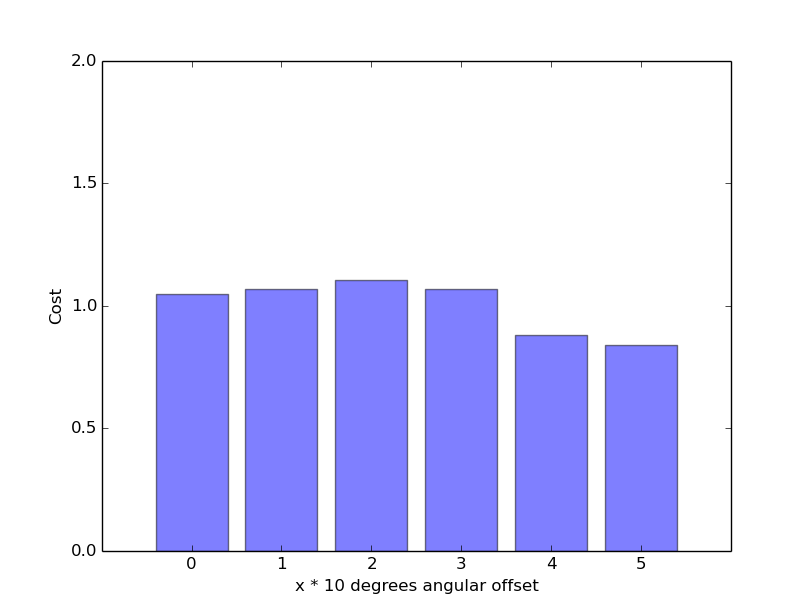
\includegraphics[width=\textwidth]{figures/cost_twente_data.png}
        \caption{Social cost vs. Individual bearing state}
        \label{fig:cost_twente_1}
    \end{subfigure}
    \begin{subfigure}[b]{0.45\textwidth}
        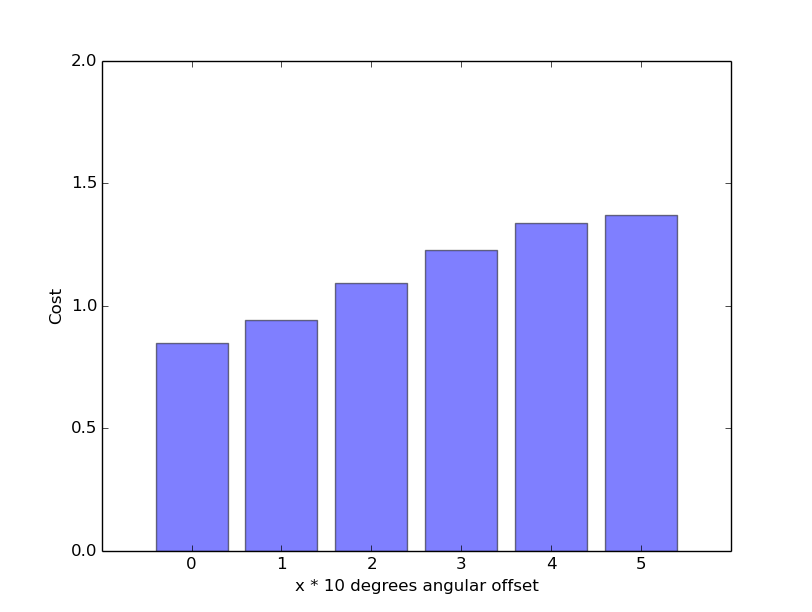
\includegraphics[width=\textwidth]{figures/cost_twente_data_COM.png}
        \caption{Social cost vs. Group bearing state}
        \label{fig:cost_twente_2}
    \end{subfigure}
    \caption[Social cost based on bearing.]{Social cost based on bearing w.r.t. (\subref{fig:cost_twente_1}) each individual participant and (\subref{fig:cost_twente_2}) with respect to the geometric center of the group.}
    \label{fig:social_cost_function_twente}
\end{figure}

Equipped with this result we have extracted a measure of social cost as a funtion of the bearing state with respect to the geometric center of the group, based on the probability of receiving an error-free score (score $7$) in each state. This function is represented in Figure \ref{fig:cost_twente_2}, and shows an almost linear increase in cost w.r.t. the deviation in bearing. As a final note, and as a way of further confirming that the individual bearing state of each participant is not a useful feature, we have also attempted to extract an analogous measure of cost as a function of this variable. The results are shown in Figure \ref{fig:cost_twente_2}, and show a \emph{decrease} in cost as the deviation in bearing increases (which would lead to incorrectly rewarding behaviours for having higher bearings).

\section{Conclusions and Future Work in Tasks 5.1 and 5.2}
\label{sec:conclusions}
This deliverable has summarised our progress for Work Package 5 from month 15 of the project until month 30. Significant progress has been achieved in all aspects of social behaviour learning on the TERESA robot. 

 An important aspect of this progress is in terms of learning from human demonstrations, using IRL. Firstly we have enabled the robot to learn from failed demosntrations as well as succesful ones in a unified principled framework. We have demonstrated that our method is capable of utilising the failed demonstrations in conjunction with the succesful ones to learn faster and better. Secondly we have developed a novel IRL method called, RLT$^*$ that works with RRT$^*$ as the underlying planner. RRT's are at the heart of TERESA's path planning module, thus learning directly using this planners is bound to produce superior learning results. We have also shown that our method is faster and better that a similar method that uses deterministic planners. A clear avenue of future work is to deploy RLT$^*$ on the real system. Furthermore we plan to integrate these methods together and evaluate any improvement on the real system.

 We have also reported significant progress in terms of experimentation and implementation of social conversation policies. Specifically, we conducted experiments and performed the necessary analysis, in order to discover a cost function for the distance between the robot and the interaction target. In addition we performed statistical analysis on an existing dataset gathered by our partners at UT. This dataset consisted of groups of people scoring how well the TERESA robot approached them. This analysis allowed us to produce a second cost function that determines how the robot should be orientated in such situations. The analysis also concluded that the bearing of the robot to the group's geometric centre was far more important to the bearing with respect to an individual person. This allowed us to determine a compact yet representative state-space representation for the robot during conversation. 

 In terms of social conversation, there are two directions of future work we are currently pursuing and for which we plan to report in month 36. Firstly we aim to integrate these cost functions in order to learn a single social conversation policy under which the robot operates. Secondly we aim to make the resulting policy more robust to false positives from the robots social detectors using advances filtering techniques such as Partially Observable Markov Decision Processes (POMDPs) and Long-Short Memory Networks (LSTMs).




\bibliographystyle{plain}
\bibliography{references}

\end{document}
